\documentclass{article}
\usepackage{fullpage}
\usepackage{verbatim}
\usepackage{graphicx}
\usepackage{hyperref}
\usepackage{pdflscape}
\usepackage{caption}
\usepackage{longtable}
\usepackage{color}


\renewcommand{\arraystretch}{1.5}
\captionsetup[table]{name=Design Decision,font={large,sf}}
\begin{document}
\title{Software Architecture}
\author{Chiel Peters, Omar Pakker, Mary Gouseti, Cindy Berghuizen}
\maketitle

\tableofcontents

\setlength\parindent{0pt}

\section{Introduction}
\subsection{Scope And Summary}
This document provides the current architecture of the FlyWithUs application. FlyWithUs is a new start-up that wants to create a single platform for airlines and users to write and read flight reviews. The platform must combine reviews from other sites as well as reviews from within the FlyWithUs application.
This document identifies the stakeholders, requirements, design decisions and viewpoints on the current architecture of the FlyWithUs application and contains an overall definition of architecture. Because FlyWithUs does not currently have any technical employees (developers, testers etc.) these stakeholders are currently left out of scope of this document.
 
\subsection{Viewpoint Overview}
The document contains three viewpoints on the architecture:
\begin{enumerate}
\item \emph{Functional Decomposition view}. This viewpoint identifies the different users within the system and their functionality. It also shows which modules are responsible for which actions.
\item \emph{Data Flow}. This viewpoint is responsible for showing how data flows through the system.
\item \emph{Concurrency view}. This viewpoint explains the performance and scalability of the system along with the tactics used to achieve those.
\end{enumerate}
 
\subsection{Document Organization}
In the first section, the stakeholders are identified together with their concerns.
The second section contains multiple viewpoints on the architecture of the FlyWithUs system. In Appendix A the requirements of the stakeholders are stated. The design decisions are given in Appendix B and finally Appendix C contains the domain related analysis.
%TODO: appendix D info needs to be inserted here

\section{Definition of Architecture}

First four definitions of software architecture are stated and their differences
and similarities are discussed. Second, our own view on software architecture is
given.
\subsection{Definitions on architectures}

\begin{enumerate}
\item Software Architecture is the set of structures needed to reason about the software system, which comprise the software elements, the relations between them, and the properties of both elements and relations.\cite{clemens}

\item Software Architecture is an abstract system specification consisting primarily of functional components described in terms of their behaviours and interfaces and component-component interconnections\cite{hayesroth}

\item Software Architecture is the fundamental organization of a system embodied in its components, their relationships to each other, and to the environment, and the principles guiding its design and evolution.\cite{IEEE1471}

\item Software architecture is the study of the large-scale structure and performance of software systems. Important aspects of a system's architecture include the division of functions among system modules, the means of communication between modules, and the representation of shared information.\cite{lane90}

\end{enumerate}

These definitions share the same fundamental idea that software architecture
is a set of structures/components/modules including their properties and the
relationships between them. However, each of the definitions highlights certain
aspects of architecture more than the others. 
\begin{itemize}
\item In \cite{clemens} and \cite{hayesroth} the focus has been put on the end result. The architecture 
is defined as the components themselves (their properties/interfaces) and the relationships between them (interconnections).
\item The definition stated in \cite{hayesroth} lays a focus on the functional components of a software architecture. With words like functional components, 
behaviours and interfaces underlines the importance of declaring the way the components interact with each other.
\item The definition of \cite{IEEE1471} is not limited only to the systems components, their functionalities and connections but also includes in the definition the 
process of designing and maintaining an architecture. It explicitly states that the design process and the evolution are part of the architecture itself.
\item The last definition (\cite{lane90}) presents architecture as the study of a system's structure. As a result architecture contains the modules and the connections between them that build the system. This also becomes clear
from the title of the article \emph{Studying Software Architecture Through Design Spaces and Rules}.

\end{itemize}

\subsection{Our view on architecture}
As the definitions mentioned above, we also agree on the point that a software architecture is defined as a set of components, their properties, behaviours and the relations
between. However, we think that architecture is not only the structure of a software system but also contains the main design decisions that would explain why the system consists of 
these components and include the stakeholders' quality attributes that lead the architects to those decisions. \\ 

Our definition of software architecture would be:
Software architecture is the structure of a software system along with the decisions that lead to this structure. To elaborate, architecture contains the components by which
the system is build up, their functionality, the relations between them and the reason of their existence meaning which requirement of the stakeholders or quality attribute they accomplish. 

%Stakeholder part
\section{Stakeholder Concerns}

In this project there are four different stakeholder :
\begin{enumerate}
\item The Initiator
\item AirFrance - KLM
\item The Dutch Government
\item EU Claim
\end{enumerate}

Each of them had different concerns within this project which are stated in the next subsections.

\subsection{Initiator}
The initiator is the one who started this project. He wants FlyWithUs to be a success and become the number one rating site people will go to. He want to be able to collect data from social media, other rating websites, news, weather and every other source that can be of importance. This data an then be used to provide the airlines with powerfull statistics and can give users a final rating. Users that make use of FlyWithUs have to be able to post reviews and ratings on the website and search for them. What makes FlyWithUs unique is the fact that airlines can get in touch with the users by sending them messages.

\subsection{AirFrance - KLM}
This stakeholder wants to have a reporting tool. With the tool he has to be able to see what recent reviews have been posted about his airline. Also, AirFrance - KLM wants to see statistics and be able to see what causes a sudden decline or increase in the rating. Furthermore, AirFrance-KLM wants to be able to enter flight information and by doing so influence the weight of review. This means that the weight of a rating has to be less when bad ratings are due to for example environmental issues (bad weather etc.) and have nothing to do with the airline companies services.

\subsection{Dutch Government}
Privacy is an important issue for the Dutch Government. The server needs to be hosted in the Netherlands so FlyWithUs will be led according to the Dutch Privacy Law. Also, the Dutch Governemnt would like to see the project to be a "Green IT" project. 

\subsection{EU Claim}
EU Claim wants to make certain that the privacy if the user is guaranteed. Furthermore the airlines have to behave on the website and do not mess with the results or bribe the users. Fairness is thus also an important issue to this stakeholder.

%Input viewpoints here
\section{Viewpoints}
%TODO: This block requires changing
This section contains three viewpoints on the architecture. These viewpoints were mainly due to the stakeholders concerns. The privacy view provides EU-Claim and the Dutch government the information related to their main concerns. The data-flow indicates how the system will be able to handle all the data from external and internal sources which is one of the biggest challenges in designing this architecture. The last view shows the functional requirements of the system of all the available users.

% \input{Functional}

\subsection{Functional Viewpoint}

\begin{itemize}
\item Related stakeholders: KLM, Initiator, EU-Claim
\item Related Concerns: Users of the system, Available functionality to each user group, Grouping functionalities
\item Related design decisions: EU-Claim can see private conversation after invitation \ref{}, Billing system added \ref{}, Functionalities of Reporting System\ref{}.
\end{itemize}

\newpage
\begin{landscape}
\begin{figure}
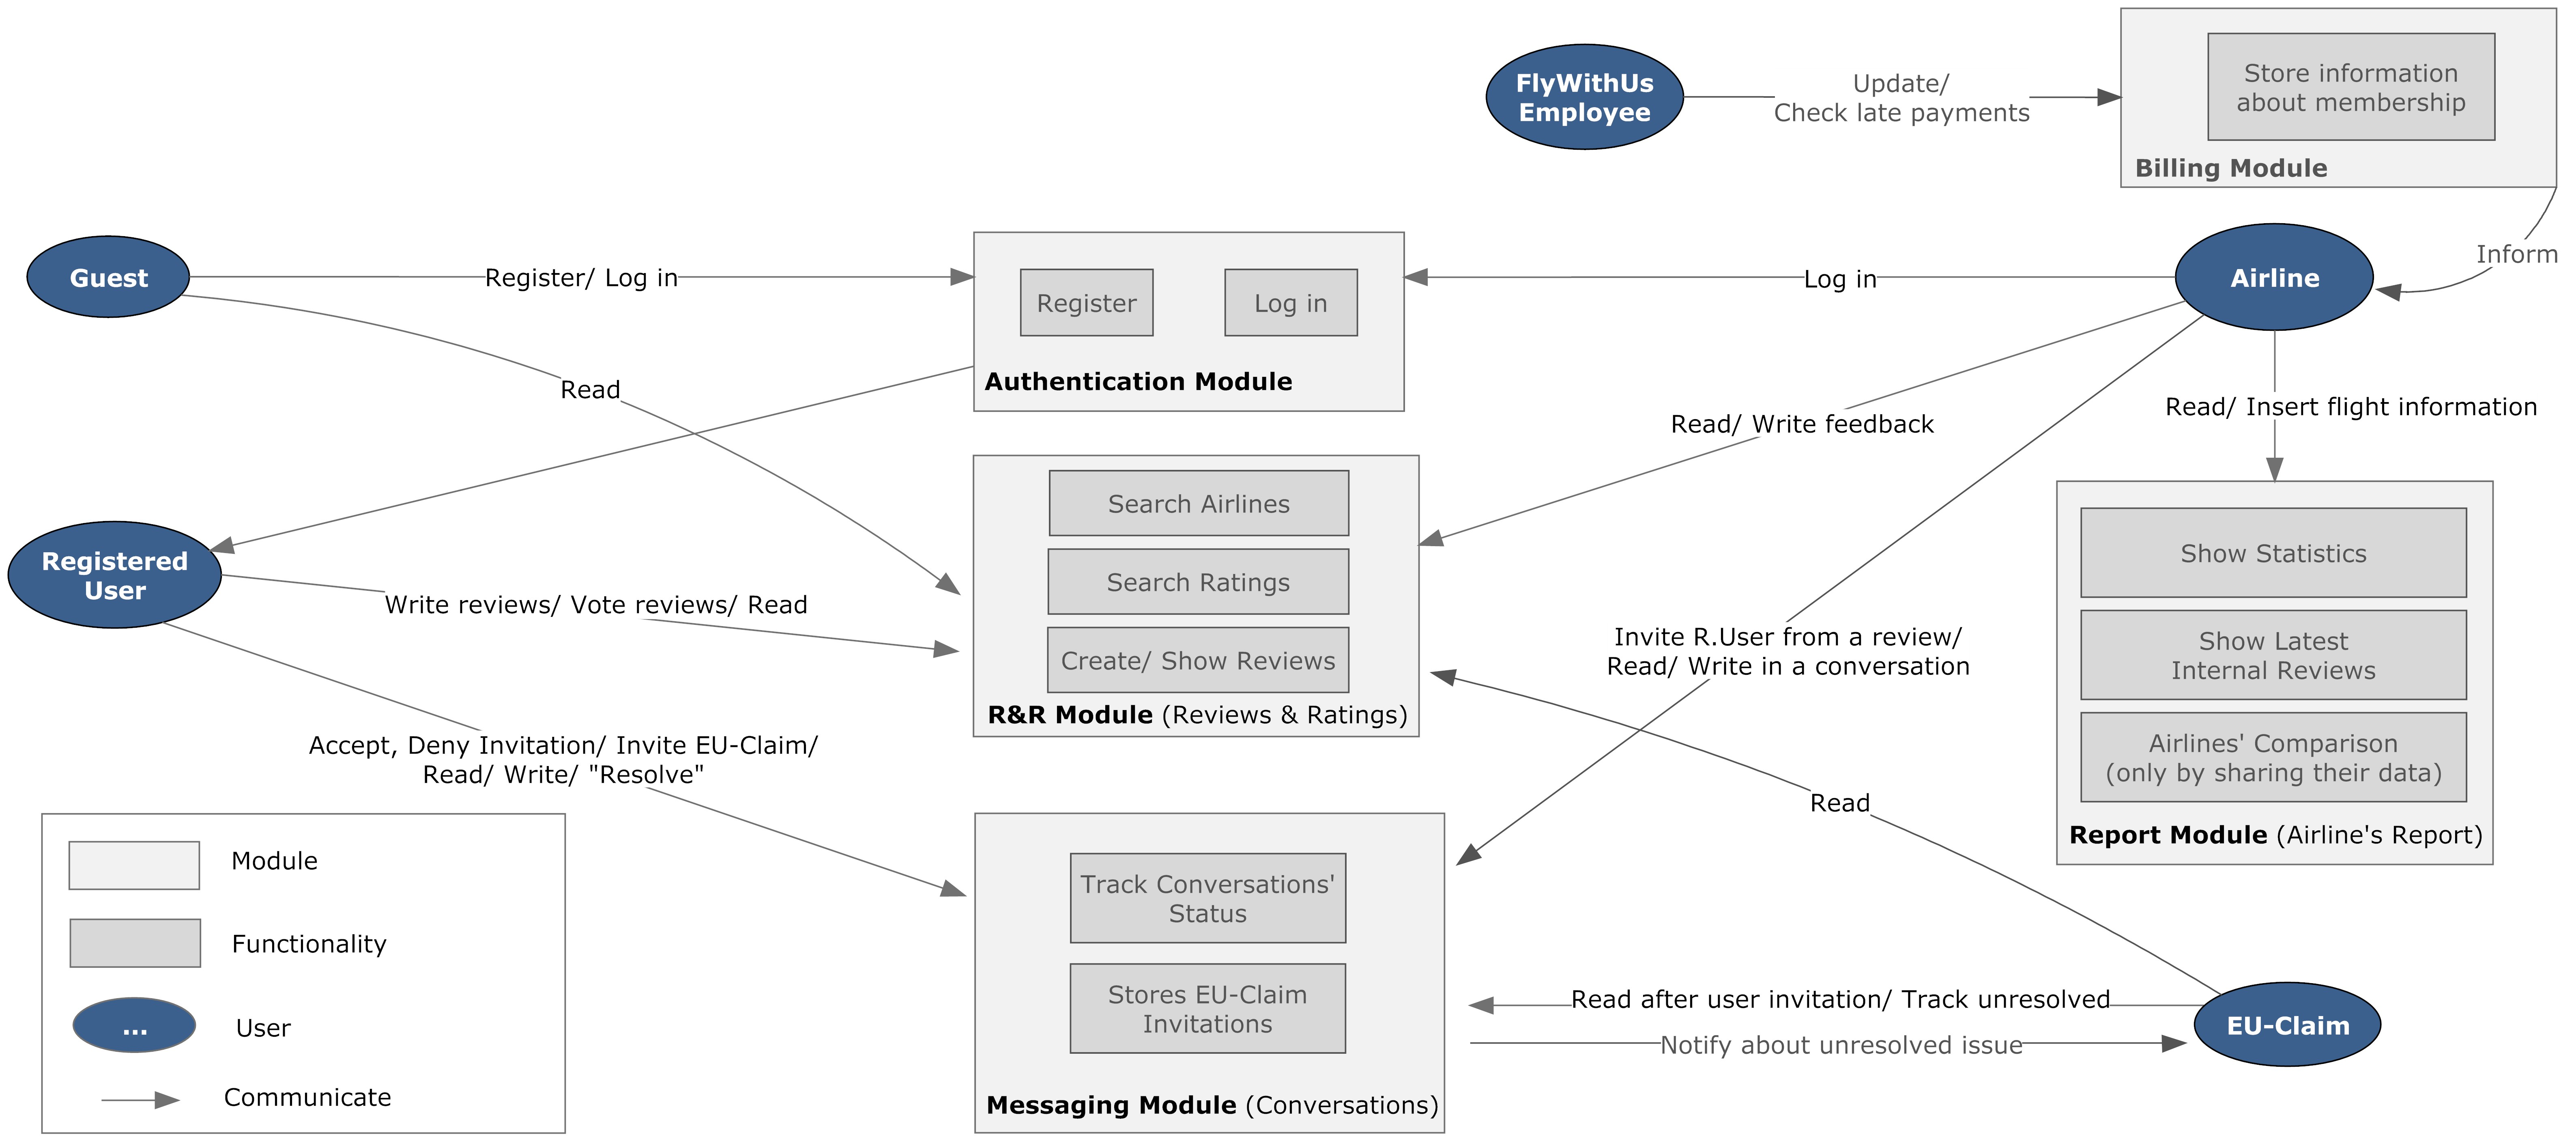
\includegraphics[width=600px]{Functional_Viewpoint.jpg}
\caption{Functional Viewpoint}
\label{fig:functional}
\end{figure}
\end{landscape}

The functional viewpoint (Fig.~\ref{fig:functional}) illustrates the functionality supported by the system and its connections to the users. The direction of the arrows shows who or what initiates this connection, for example EU-Claim can monitor a conversation (initiated by EU-Claim) but  the system notifies EU-Claim about an issue that has been unresolved for a configurable period of time (initiated by Messaging module). The functionalities that are based in the same entities of the system are grouped together to help the reader understand their connections. For example, all the functionalities  provided only to airlines are included in a {\em report} as a result these functionalities are grouped in the Report module. The association between the modules presented in the viewpoint and the functional requirements listed in table~\ref{requir} is shown in table below:
%TODO: Fix reference

\begin{longtable}{| l | l | l |}
\hline
\label{tab:associateSysReq} 
\textbf{Requirement} & \textbf{System} & \textbf{Users} \\ \hline
Show ratings & Review System & Guests, Registered Users \\ \hline
Post/Read/Search/Vote & Review System & Registered Users \\ \hline
Messaging & Messaging System & Registered Users, Airlines, EUC \\ \hline
Reporting  & Reporting System & Airlines \\ \hline
Flight Information & Reporting System & Airlines \\ \hline
Statistics & Reporting System & Airlines \\ \hline 

\end{longtable}

Furthermore, the viewpoint also presents the availability of the functionalities to each user group and the communication between these groups through the system. For instance, a guest can register or log in the system and  become a registered user, or an airline can invite a user to a private conversation in order to resolve a potential complaint; then the user can accept the invitation and he can  also invite EU-Claim to monitor their conversation to ensure the integrity of this process.

Each entity presented in the viewpoint is discussed in the following sections.

\subsubsection{Users}
\paragraph{Guests.} A guest is a user of our system with no account. He can read reviews and search for ratings using the R\&R module. Furthermore, a guest can  register or log in the Authentication module.
\paragraph{Registered User.} A registered user can read, write and vote reviews and search for rating using the R\&R module. Additionally, he can communicate with an airline through the Messaging module in private, meaning that other parties  (except for EU-Claim and only if it is invited) cannot read this conversation.
\paragraph{Airlines.} An airline represents the airlines that have payed membership in FlyWithUs. An airline can monitor its progress checking the Report module. Also an airline can see statistics, ratings and search according to flight information it can provide. 

Additionally, as far as customer satisfaction is concerned, an airline can write feedback to a review posted on the R\&R module or invite a user to a private conversation through the Messaging module.

Finally, it can be informed about the status of its membership thought the Billing module.

\paragraph{EU-Claim.} In order to ensure the integrity of the system, EU-Claim will have separate accounts that will enable her to monitor conversations when she is invited and also notify her of a conversation is unresolved for a configurable period of time.

\paragraph{FlyWithUs Employee.} FlyWithUs employee is an employee of FlyWithUs whose responsibility is to update or check the membership status of the airline according to their payments.

\subsubsection{Modules}
\paragraph{Review \& Rating Module.} This module is responsible for inserting new internal reviews on the system, vote reviews and provides the search interface to the registered users and guests. This module allows searching according to specific rating fields for example which airline has the best food or the best client support, or according to general ratings. 

The R\& R module does not allow the users to  edit or delete their rating in order to preserve the system's consistency and integrity.

\paragraph{Report Module.} This module provides the tools to the airlines to monitor their progress. It shows statistics about the airline progress, the latest reviews on FlyWithUs and also allows the airlines to use advance search, which enables them to insert flight information or other parameters and search through our database.

\paragraph{Messaging Module.} This module is responsible for the private conversations between the registered users and the airlines. At first, an airline declares that wishes to contact the author of a review, then the author is invited to a private conversation. If the author accepts it can invite EU-Claim to monitor this conversation through this module. Additionally, this module keeps track of all the resolved and unresolved issues, it can provide statistics and it can also notify EU-Claim if a conversation has been unresolved for a configurable (by EU-Claim) period of time. Only the affiliated parties of a conversation can read this conversation as a result the Messaging module checks the identity of the user before it grants him access.

\paragraph{Billing Module.} This module is responsible for keeping track of the membership status of the airlines. It will notify both the FlyWithUs employee and the associated airline if there is a late payment and in case that the airline's membership is not renewed it will revoke the airline's access to the Reporting module.

\paragraph{Authentication Module.} This module is responsible for the registration of new users and for signing in existing users and identifying their type.

%% % % \input{PrivacyView}

\subsection{Privacy viewpoint}

\begin{itemize}
\item Related stakeholders: Dutch government, EU Claim
\item Related Concerns: Privacy of the user
\end{itemize}

\newpage
\begin{landscape}
\begin{figure}
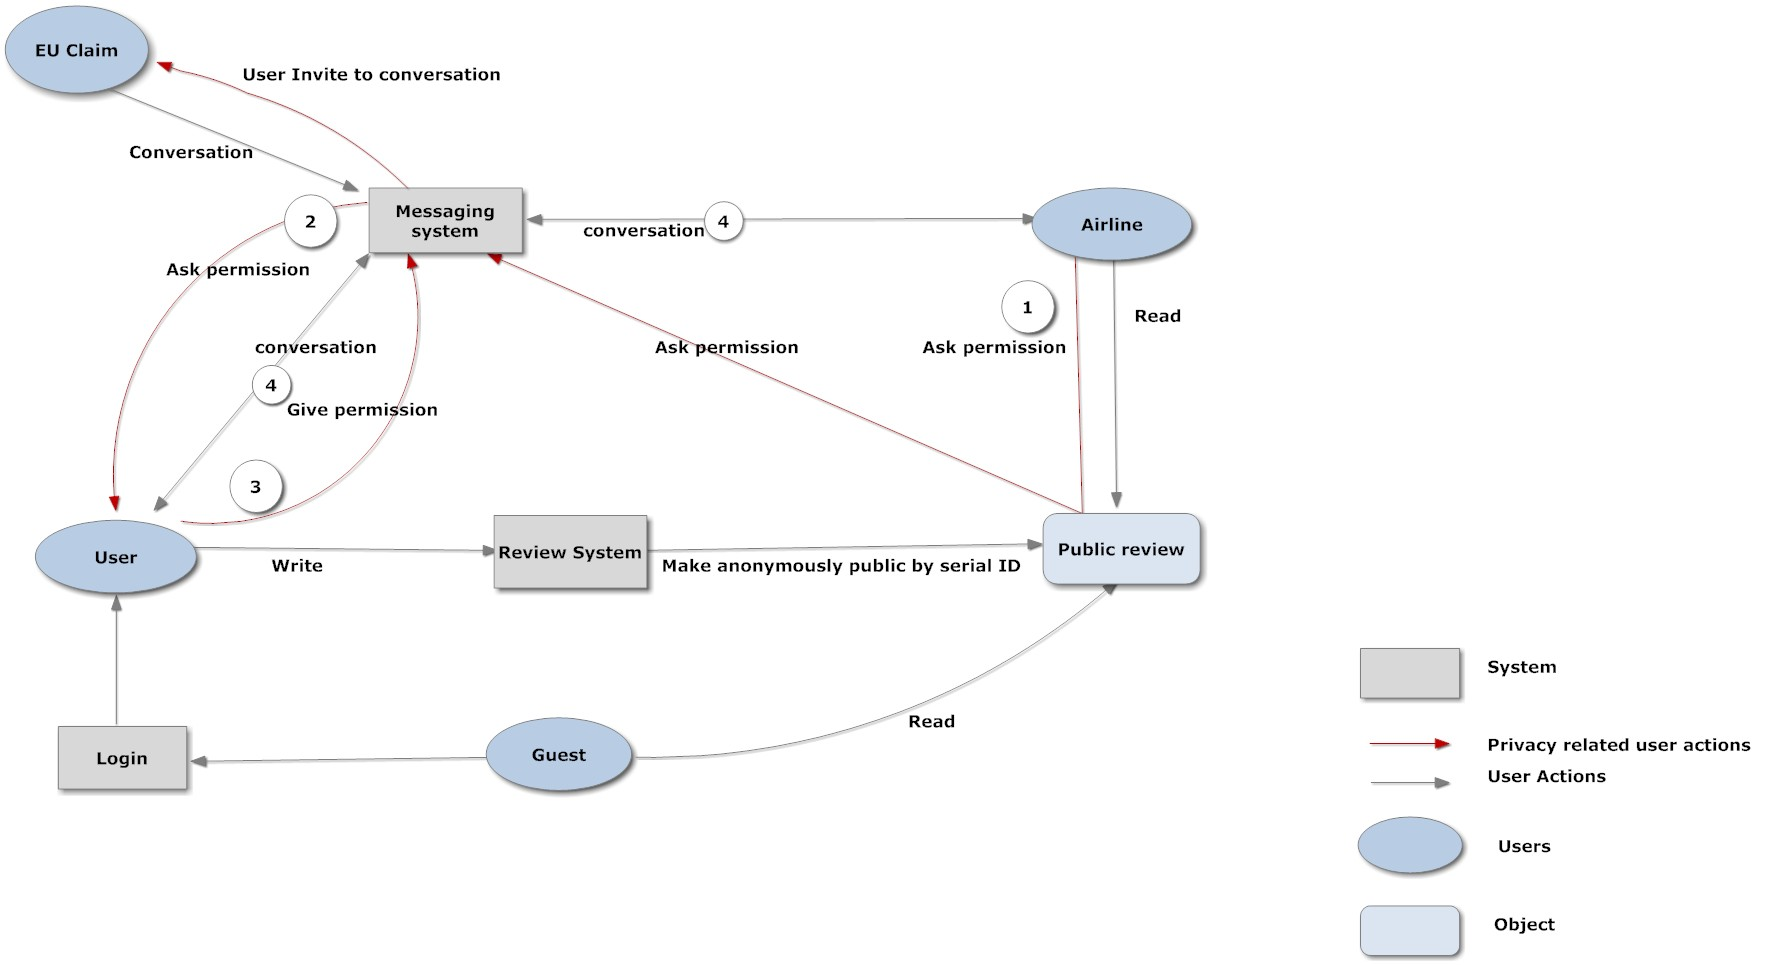
\includegraphics[width=680px]{privacyview}
\caption{Privacy viewpoint}
\label{fig:privacy}
\end{figure}
\end{landscape}
The privacy viewpoint in figure \ref{fig:privacy} shows how the privacy of the user is guaranteed in the system. A user can write a review that is shown to the public anonymously. The review will have a serialID instead of the user name so the user will stay unknown to the public. 

An airline should be able to have a conversation with an user if the airline wants to elaborate on a specific case or wants to adress the user personally. If the airline wants to get the user's information for a conversation it should ask permission of the user. When a user accepts to have a conversation with an airline the user's contact information is visible to the airline so they will be able to have a conversation. If the user is not satisfied with how the airline company responds on requests or remarks in the conversation, the user is able to invite EU Claim to the conversation so they will be able to see the conversation and decide to act upon it.

\subsection{Privacy viewpoint}

\begin{itemize}
\item Related stakeholders: Dutch government, EU Claim
\item Related Concerns: Privacy of the user
\end{itemize}

\newpage
\begin{landscape}
\begin{figure}
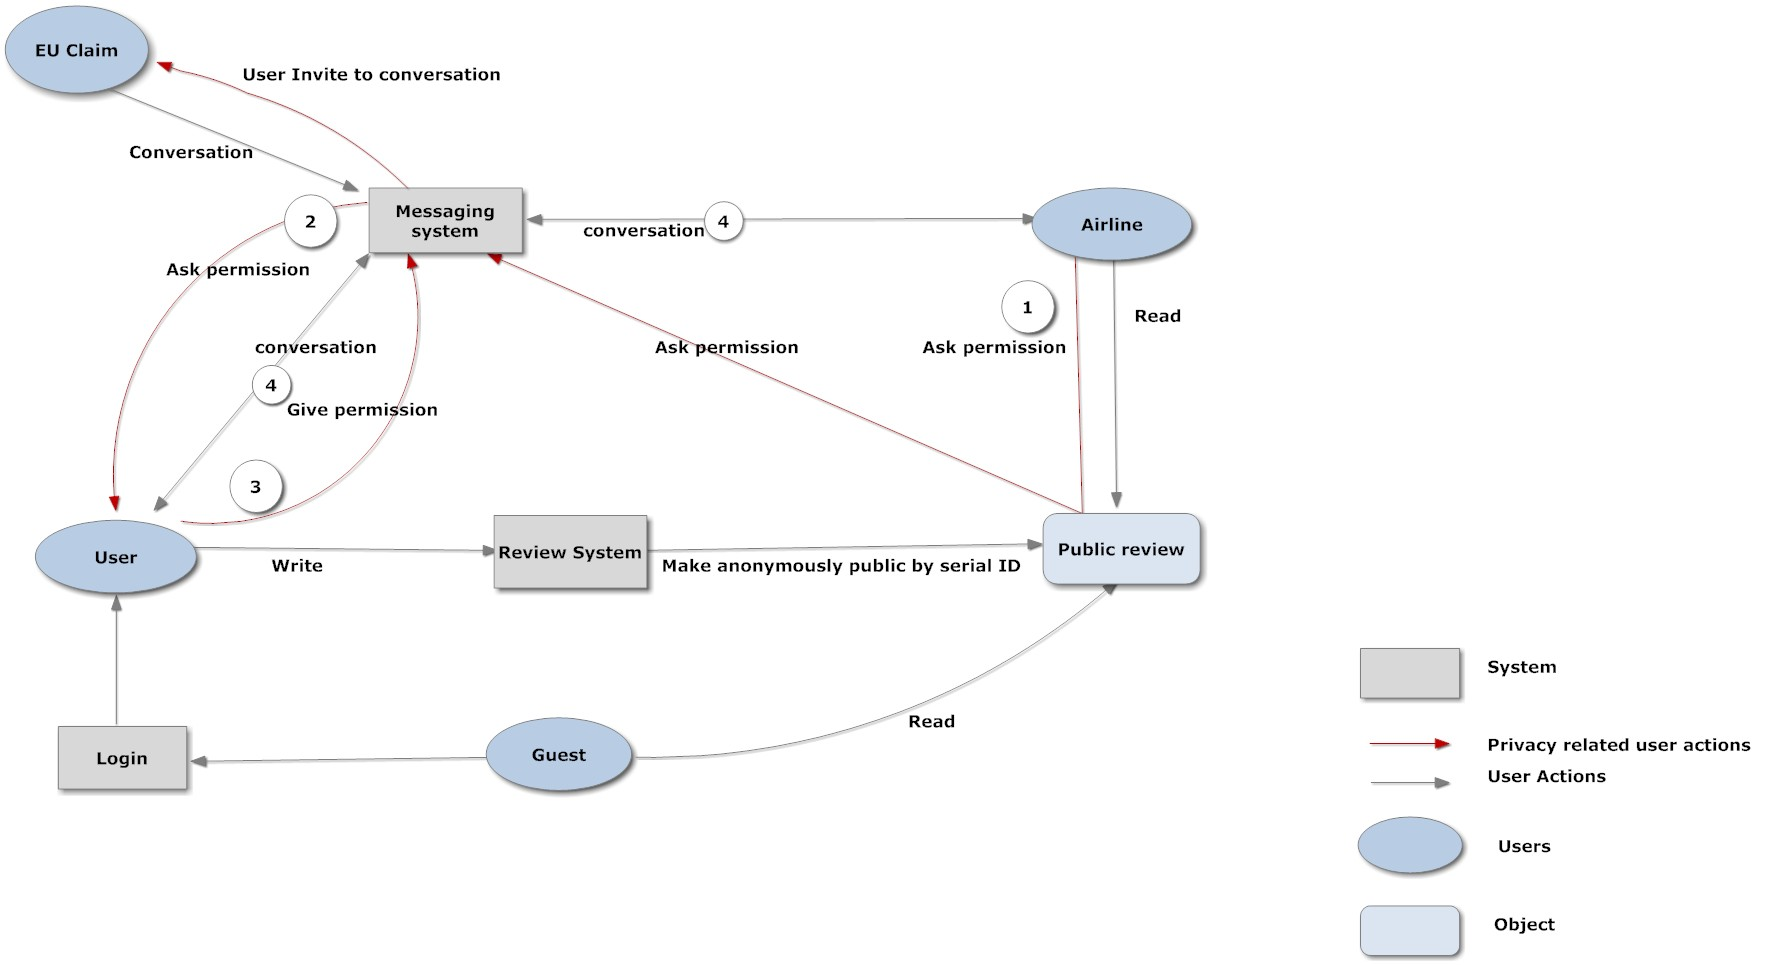
\includegraphics[width=680px]{privacyview}
\caption{Privacy viewpoint}
\label{fig:privacy}
\end{figure}
\end{landscape}
The privacy viewpoint in figure \ref{fig:privacy} shows how the privacy of the user is guaranteed in the system. A user can write a review that is shown to the public anonymously. The review will have a serialID instead of the user name so the user will stay unknown to the public. 

An airline should be able to have a conversation with an user if the airline wants to elaborate on a specific case or wants to adress the user personally. If the airline wants to get the user's information for a conversation it should ask permission of the user. When a user accepts to have a conversation with an airline the user's contact information is visible to the airline so they will be able to have a conversation. If the user is not satisfied with how the airline company responds on requests or remarks in the conversation, the user is able to invite EU Claim to the conversation so they will be able to see the conversation and decide to act upon it.

\subsection{Privacy viewpoint}

\begin{itemize}
\item Related stakeholders: Dutch government, EU Claim
\item Related Concerns: Privacy of the user
\end{itemize}

\newpage
\begin{landscape}
\begin{figure}
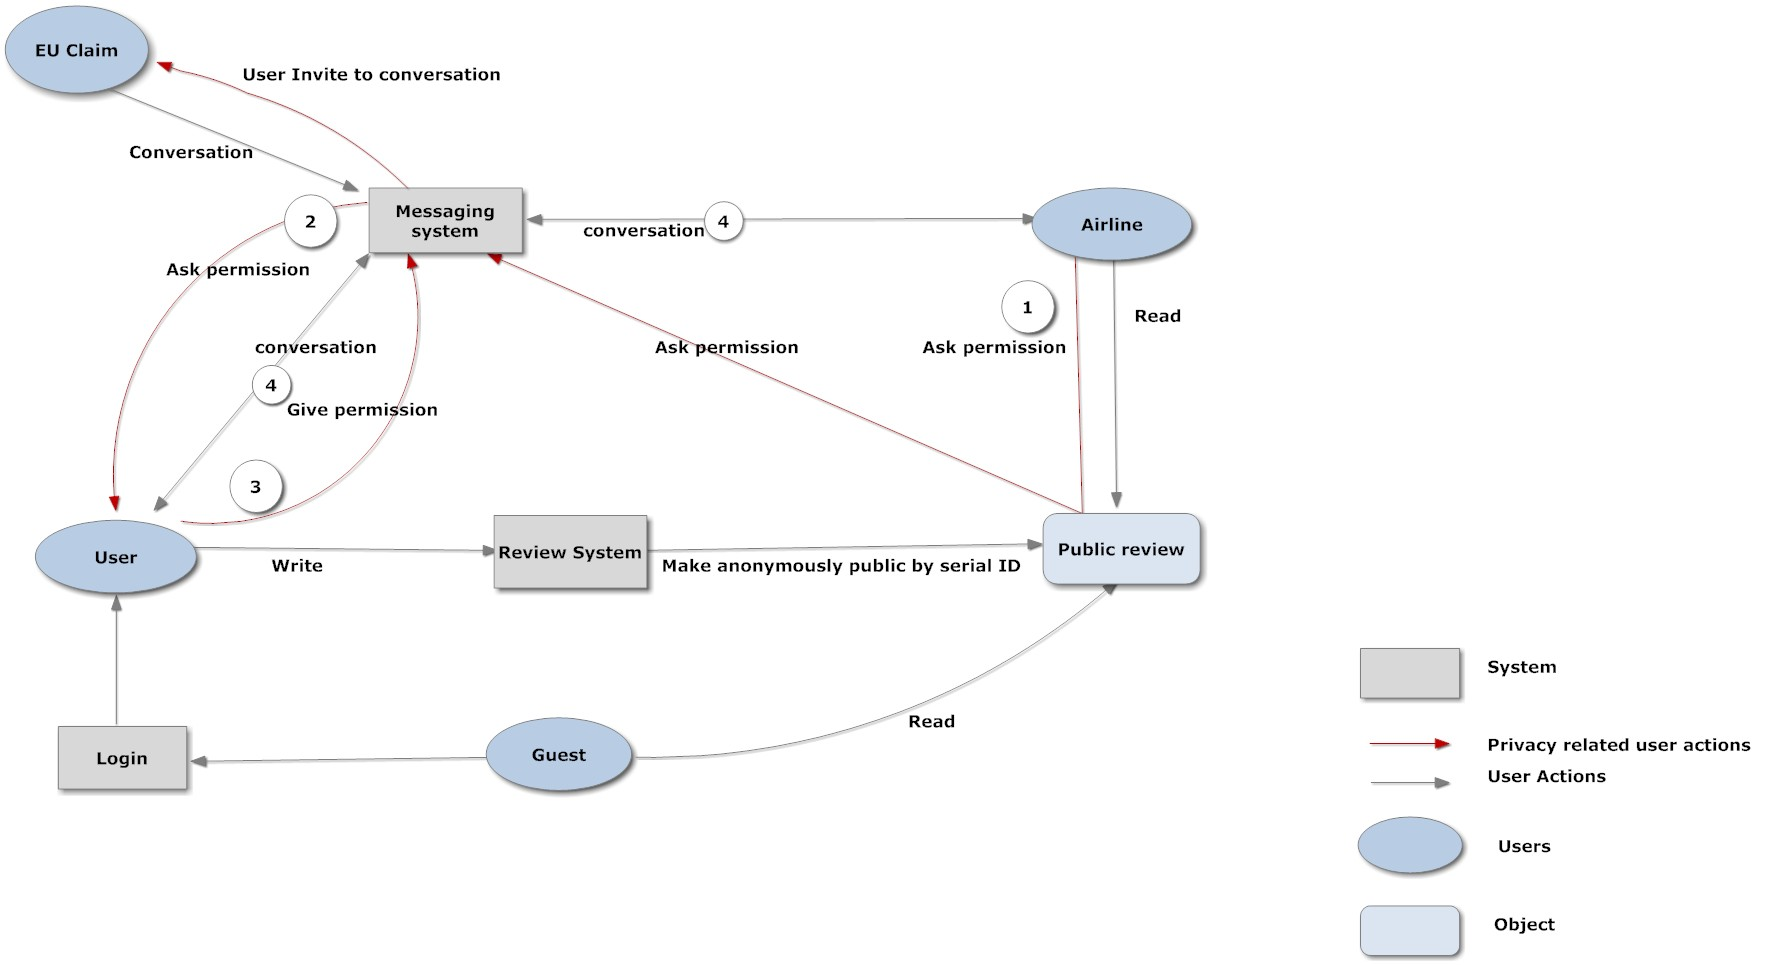
\includegraphics[width=680px]{privacyview}
\caption{Privacy viewpoint}
\label{fig:privacy}
\end{figure}
\end{landscape}
The privacy viewpoint in figure \ref{fig:privacy} shows how the privacy of the user is guaranteed in the system. A user can write a review that is shown to the public anonymously. The review will have a serialID instead of the user name so the user will stay unknown to the public. 

An airline should be able to have a conversation with an user if the airline wants to elaborate on a specific case or wants to adress the user personally. If the airline wants to get the user's information for a conversation it should ask permission of the user. When a user accepts to have a conversation with an airline the user's contact information is visible to the airline so they will be able to have a conversation. If the user is not satisfied with how the airline company responds on requests or remarks in the conversation, the user is able to invite EU Claim to the conversation so they will be able to see the conversation and decide to act upon it.
% % % \input{DataFlow}

\subsection{Data Flow Viewpoint}

\begin{itemize}
\item Related stakeholders: KLM, Initiator
\item Related Concerns: Data Integrity, Performance, Scalability
\item Related design decisions: How is the data split up into multiple databases?; How do we handle large data-sets?; Recalculate or Combine rating?; Incremental or Time-interval update?; Flight-Information
\end{itemize}

\newpage
\begin{landscape}
\begin{figure}
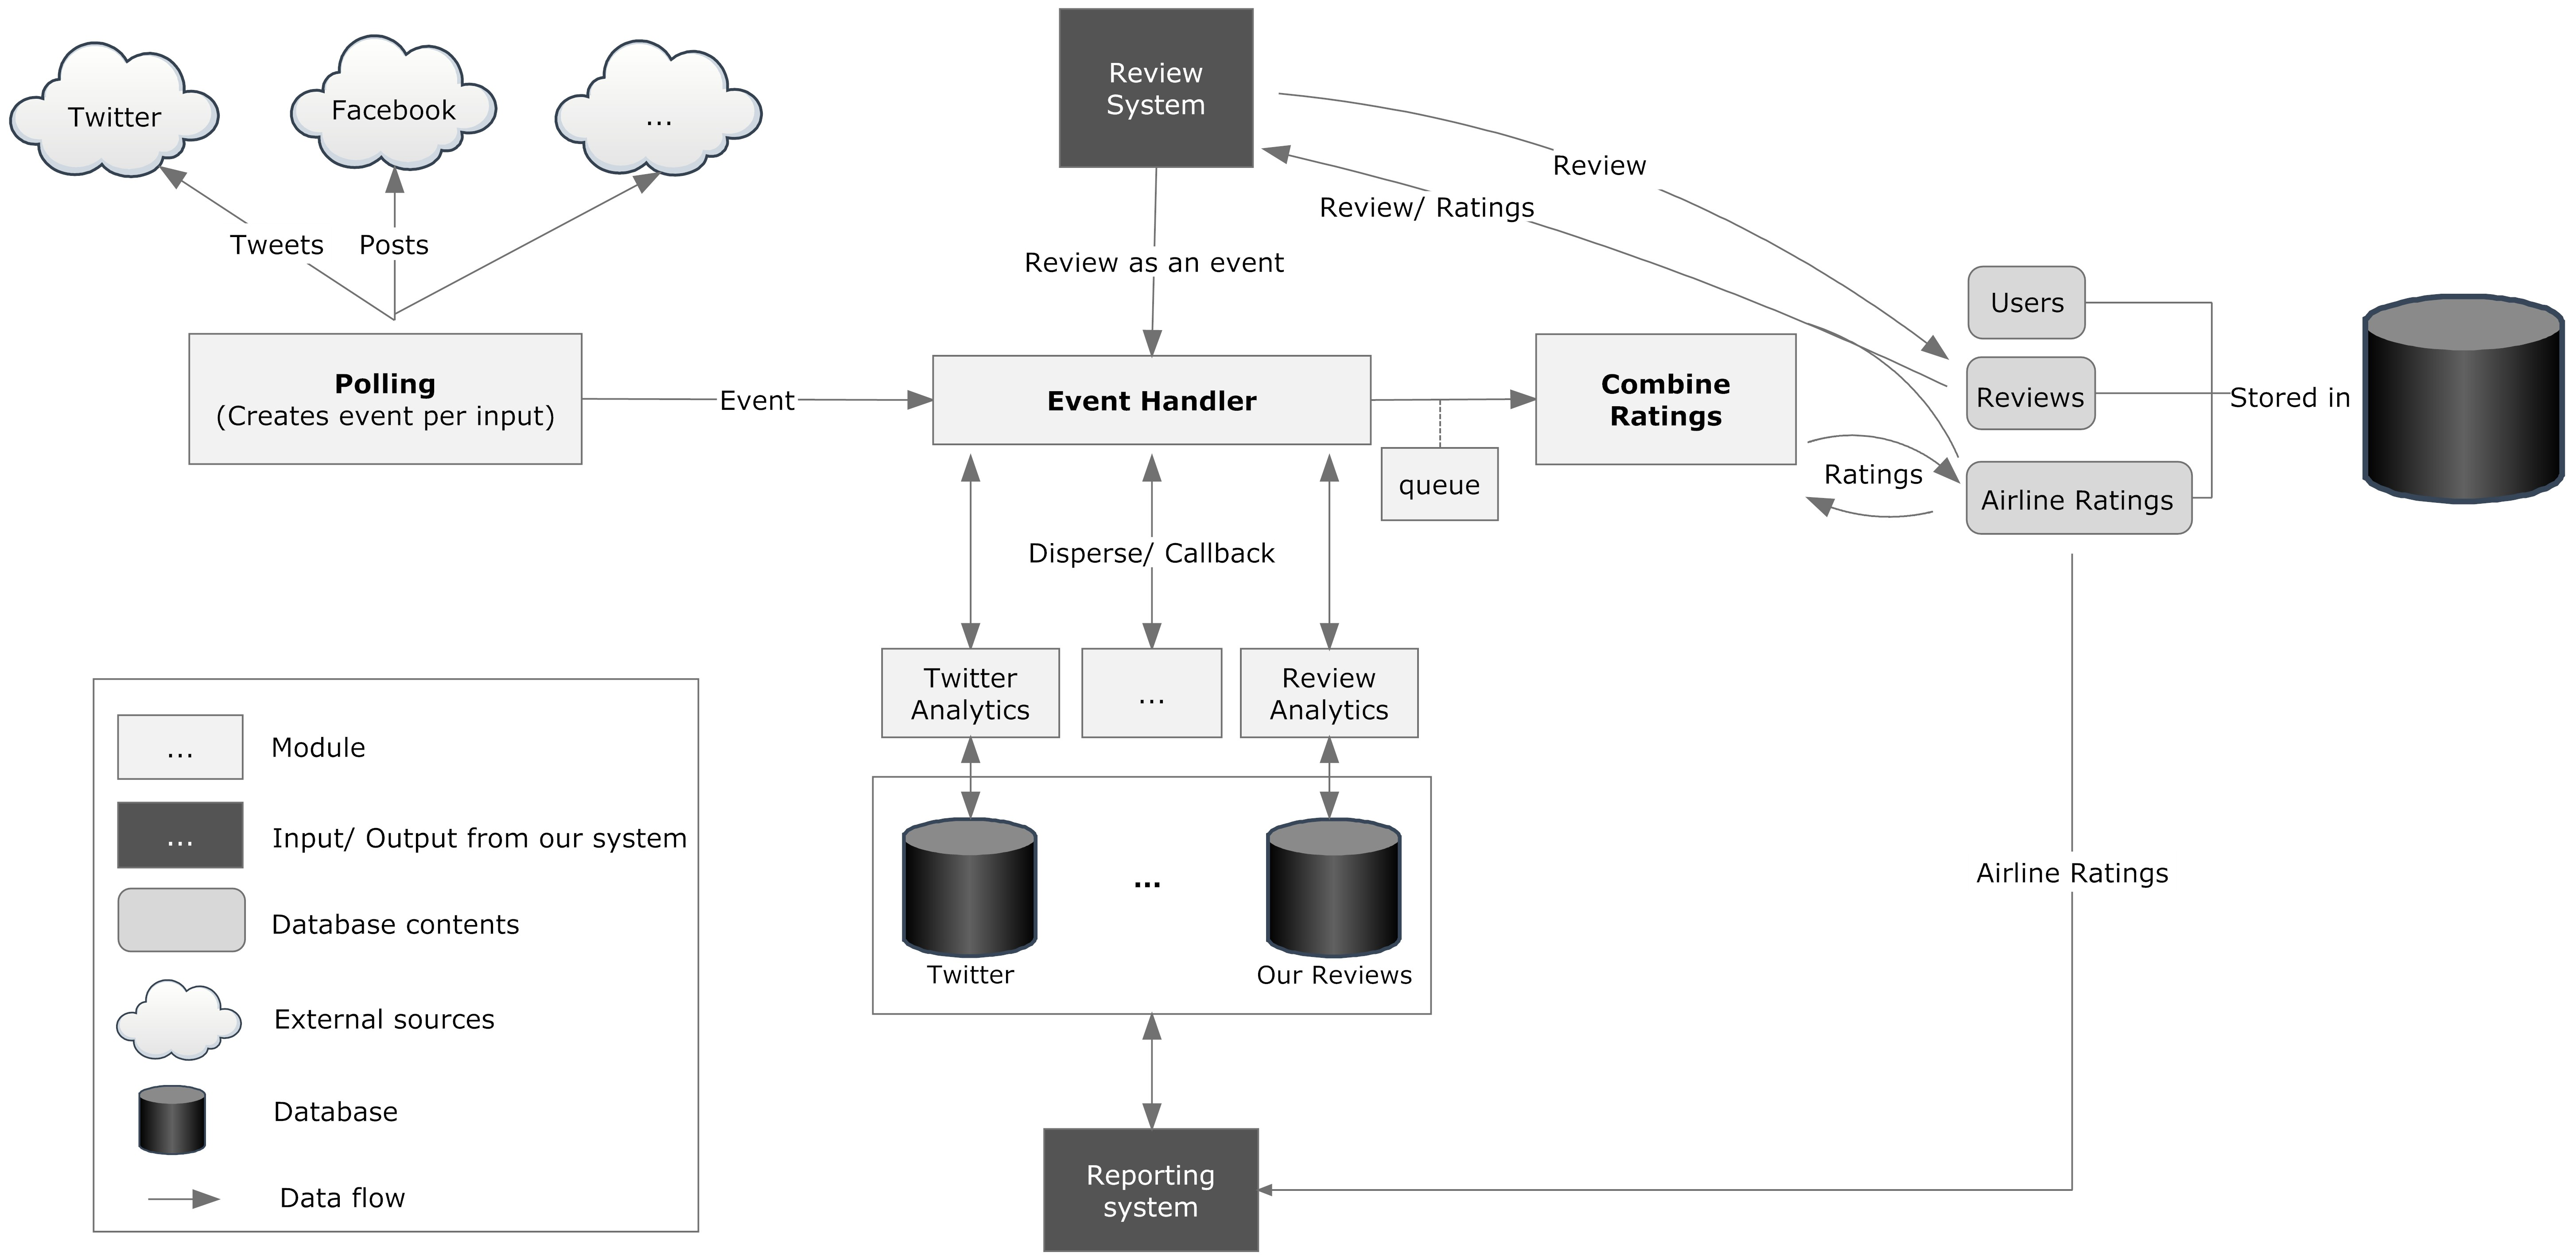
\includegraphics[width=600px]{DataFlowGraph}
\caption{Data Flow Viewpoint}
\label{fig:Data Flow}
\end{figure}
\end{landscape}

This Data Flow viewpoint \ref{fig:Data Flow} illustrates the flow of data within the back-end of the system. In this picture the review and reporting system are shown as black boxes to illustrate that their functionality is of no importance in this picture.
In the related design decisions it was argued that combining the rating with incremental updates was best for performance and scalability. Note that in the flow only the back-end of the system is given, because of the importance of handling the large data sets. Each of the modules and arrows in the viewpoint are explained here after.

\subsubsection{Polling}
The polling module is responsible for obtaining reviews from external data sources. It polls every external source on a given time-frame which is different for each external source. The reviews are not formatted and there original data format from the external source is kept. The rationale behind this decision is that all the reviews from external sources are significantly different of each other. Parsing them into a general format would lead to data loss or lots of undefined fields. The decision is further elaborated in the appendix at \ref{dd:save-raw}. The unformatted reviews are then passed on to the event handler as events. An event is defined as a single unformatted review either from external or internal sources.

\subsubsection{Event handler}
The event handler receives the events from both the polling module (external sources) and the review system (internal source). The responsibility of the event handler is to send these events to the analytics module specific to that data source. The event handler allows for parallel processing of reviews and greatly increased the performance and scalability compared to a more traditional pipeline model. This decision is further elaborated on in the appendix at \ref{dd:large-data}.

\subsubsection{Analytics}
Each data source has its own analytics module, because the data must be treated differently from external sources as they are of different format. The separate analytics modules have the added benefit of allowing for meta-analysis specific to a given data source. An example could be the amount of followers on twitter.

The analytics module analyses the unformatted review and produces a rating on a given scale for a certain or multiple categories (Overall, food, timeliness etc.). The unformatted review together with the analysed ratings are then stored in the analytics database of the data source. This is a requirement by the Initiator and KLM. The decision is further discussed in the appendix \ref{dd:data-format}. The ratings are also send of the combine ratings module in order to update the rating of the airline that is related to the review.

\subsubsection{Combine Ratings}
The combine ratings module is responsible for combining the ratings from the individual reviews into a final rating for an airline. The module receives the ratings from the analytics module and obtains the old rating from the main database. These two are combined in order to form a new rating. The process of iteratively combining ratings instead of recalculating is made for performance reasons as it is much cheaper and efficient to not recalculate the ratings that are already in the final rating of the airline. This decision is discussed in the appendix at \ref{dd:recalc-comb}. The ratings are based on an airline and a specific category (overall, timeliness, food etc.).

\subsubsection{Modules}
The functionality of each of the modules is discussed in the functional view. Hence in this section only the data flow regarding each of the modules is discussed:

\begin{enumerate}
\item \emph{R \& R module} A new review is inserted as event into the event handler which can pass it off to the specific analytics module. The decision was made to save the internal reviews twice: once in the main database and once when the they are analysed in the Analytics database. This allows the users to see the reviews without accessing the analytics database, but increases overhead as the same data is almost saved twice.
\item \emph{Reporting module} The reporting module retrieves information from the analytics database which contain all the analysed data together with the raw reviews. It must also be able to access the main database for the latest final ratings.
\item \emph{Authentication module} The user data for logging purposes is saved in the main database. The data contains sensitive information and is therefore encrypted.
\item \emph{Billing module} In order to make a profit airlines need to pay for their functionality. Therefore the billing module is able to read the current enlisted airlines and write to the database if the airlines have paid or not.
\item \emph{Messaging module} The messages are saved separately in the main database. Because they can contain user sensitive information (e.g. Flight numbers, names) the whole messages are saved in an encrypted form.
\end{enumerate}


\subsection{Data Flow Viewpoint}

\begin{itemize}
\item Related stakeholders: KLM, Initiator
\item Related Concerns: Data Integrity, Performance, Scalability
\item Related design decisions: How is the data split up into multiple databases?; How do we handle large data-sets?; Recalculate or Combine rating?; Incremental or Time-interval update?; Flight-Information
\end{itemize}

\newpage
\begin{landscape}
\begin{figure}
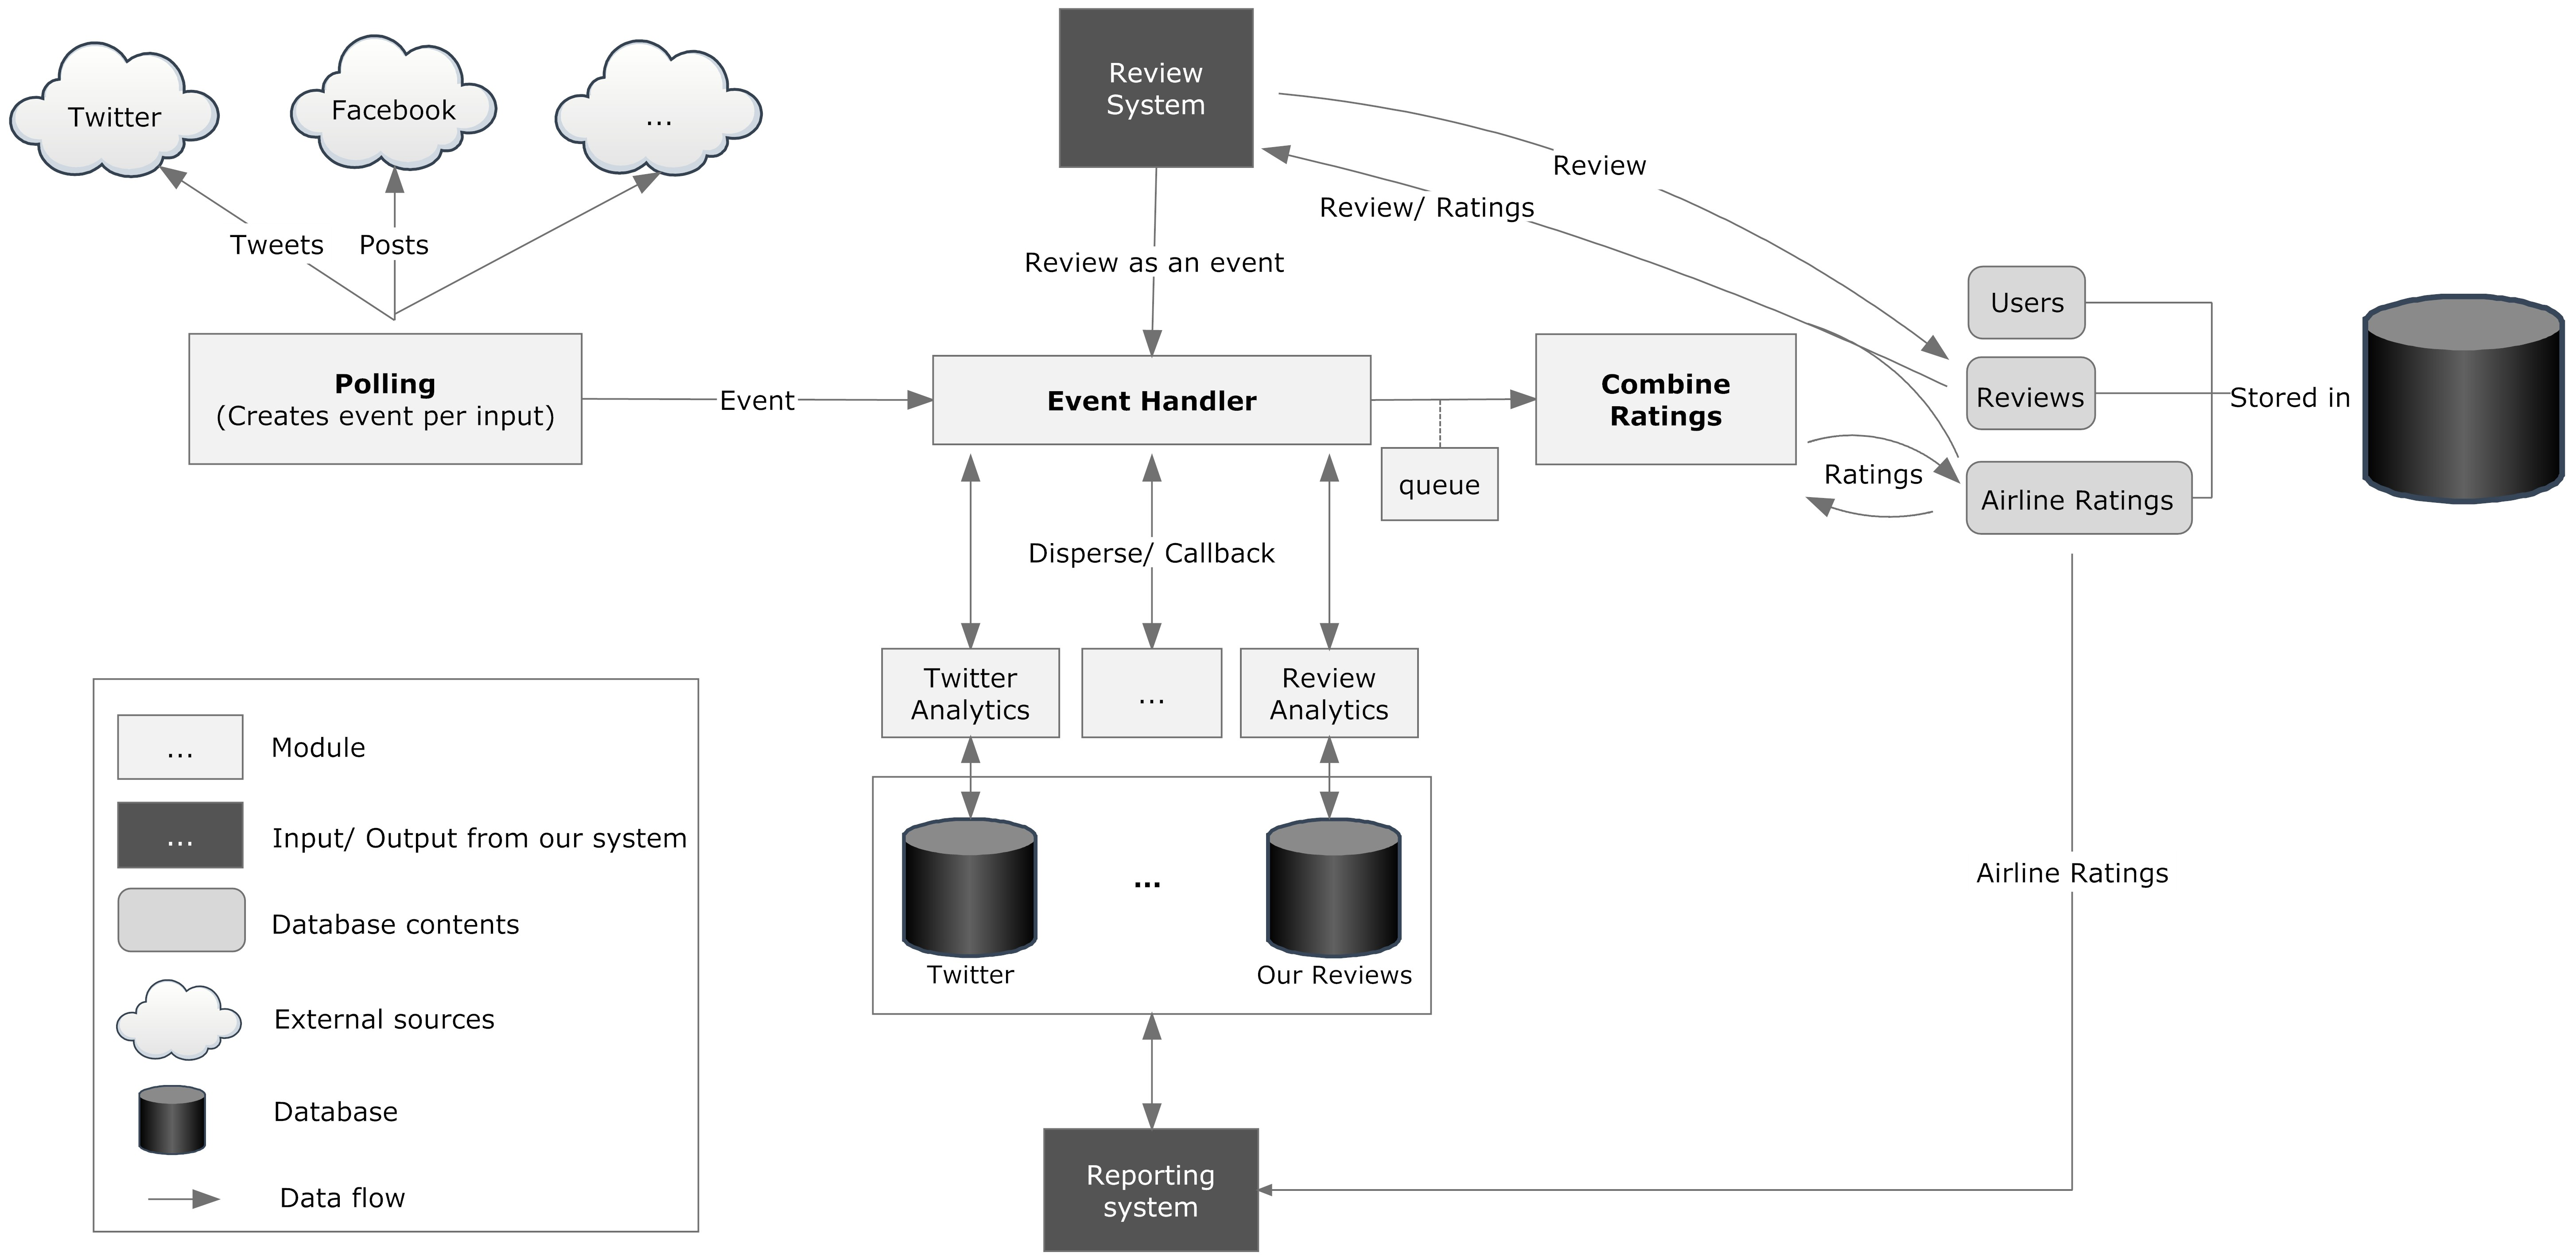
\includegraphics[width=600px]{DataFlowGraph}
\caption{Data Flow Viewpoint}
\label{fig:Data Flow}
\end{figure}
\end{landscape}

This Data Flow viewpoint \ref{fig:Data Flow} illustrates the flow of data within the back-end of the system. In this picture the review and reporting system are shown as black boxes to illustrate that their functionality is of no importance in this picture.
In the related design decisions it was argued that combining the rating with incremental updates was best for performance and scalability. Note that in the flow only the back-end of the system is given, because of the importance of handling the large data sets. Each of the modules and arrows in the viewpoint are explained here after.

\subsubsection{Polling}
The polling module is responsible for obtaining reviews from external data sources. It polls every external source on a given time-frame which is different for each external source. The reviews are not formatted and there original data format from the external source is kept. The rationale behind this decision is that all the reviews from external sources are significantly different of each other. Parsing them into a general format would lead to data loss or lots of undefined fields. The decision is further elaborated in the appendix at \ref{dd:save-raw}. The unformatted reviews are then passed on to the event handler as events. An event is defined as a single unformatted review either from external or internal sources.

\subsubsection{Event handler}
The event handler receives the events from both the polling module (external sources) and the review system (internal source). The responsibility of the event handler is to send these events to the analytics module specific to that data source. The event handler allows for parallel processing of reviews and greatly increased the performance and scalability compared to a more traditional pipeline model. This decision is further elaborated on in the appendix at \ref{dd:large-data}.

\subsubsection{Analytics}
Each data source has its own analytics module, because the data must be treated differently from external sources as they are of different format. The separate analytics modules have the added benefit of allowing for meta-analysis specific to a given data source. An example could be the amount of followers on twitter.

The analytics module analyses the unformatted review and produces a rating on a given scale for a certain or multiple categories (Overall, food, timeliness etc.). The unformatted review together with the analysed ratings are then stored in the analytics database of the data source. This is a requirement by the Initiator and KLM. The decision is further discussed in the appendix \ref{dd:data-format}. The ratings are also send of the combine ratings module in order to update the rating of the airline that is related to the review.

\subsubsection{Combine Ratings}
The combine ratings module is responsible for combining the ratings from the individual reviews into a final rating for an airline. The module receives the ratings from the analytics module and obtains the old rating from the main database. These two are combined in order to form a new rating. The process of iteratively combining ratings instead of recalculating is made for performance reasons as it is much cheaper and efficient to not recalculate the ratings that are already in the final rating of the airline. This decision is discussed in the appendix at \ref{dd:recalc-comb}. The ratings are based on an airline and a specific category (overall, timeliness, food etc.).

\subsubsection{Modules}
The functionality of each of the modules is discussed in the functional view. Hence in this section only the data flow regarding each of the modules is discussed:

\begin{enumerate}
\item \emph{R \& R module} A new review is inserted as event into the event handler which can pass it off to the specific analytics module. The decision was made to save the internal reviews twice: once in the main database and once when the they are analysed in the Analytics database. This allows the users to see the reviews without accessing the analytics database, but increases overhead as the same data is almost saved twice.
\item \emph{Reporting module} The reporting module retrieves information from the analytics database which contain all the analysed data together with the raw reviews. It must also be able to access the main database for the latest final ratings.
\item \emph{Authentication module} The user data for logging purposes is saved in the main database. The data contains sensitive information and is therefore encrypted.
\item \emph{Billing module} In order to make a profit airlines need to pay for their functionality. Therefore the billing module is able to read the current enlisted airlines and write to the database if the airlines have paid or not.
\item \emph{Messaging module} The messages are saved separately in the main database. Because they can contain user sensitive information (e.g. Flight numbers, names) the whole messages are saved in an encrypted form.
\end{enumerate}


\subsection{Data Flow Viewpoint}

\begin{itemize}
\item Related stakeholders: KLM, Initiator
\item Related Concerns: Data Integrity, Performance, Scalability
\item Related design decisions: How is the data split up into multiple databases?; How do we handle large data-sets?; Recalculate or Combine rating?; Incremental or Time-interval update?; Flight-Information
\end{itemize}

\newpage
\begin{landscape}
\begin{figure}
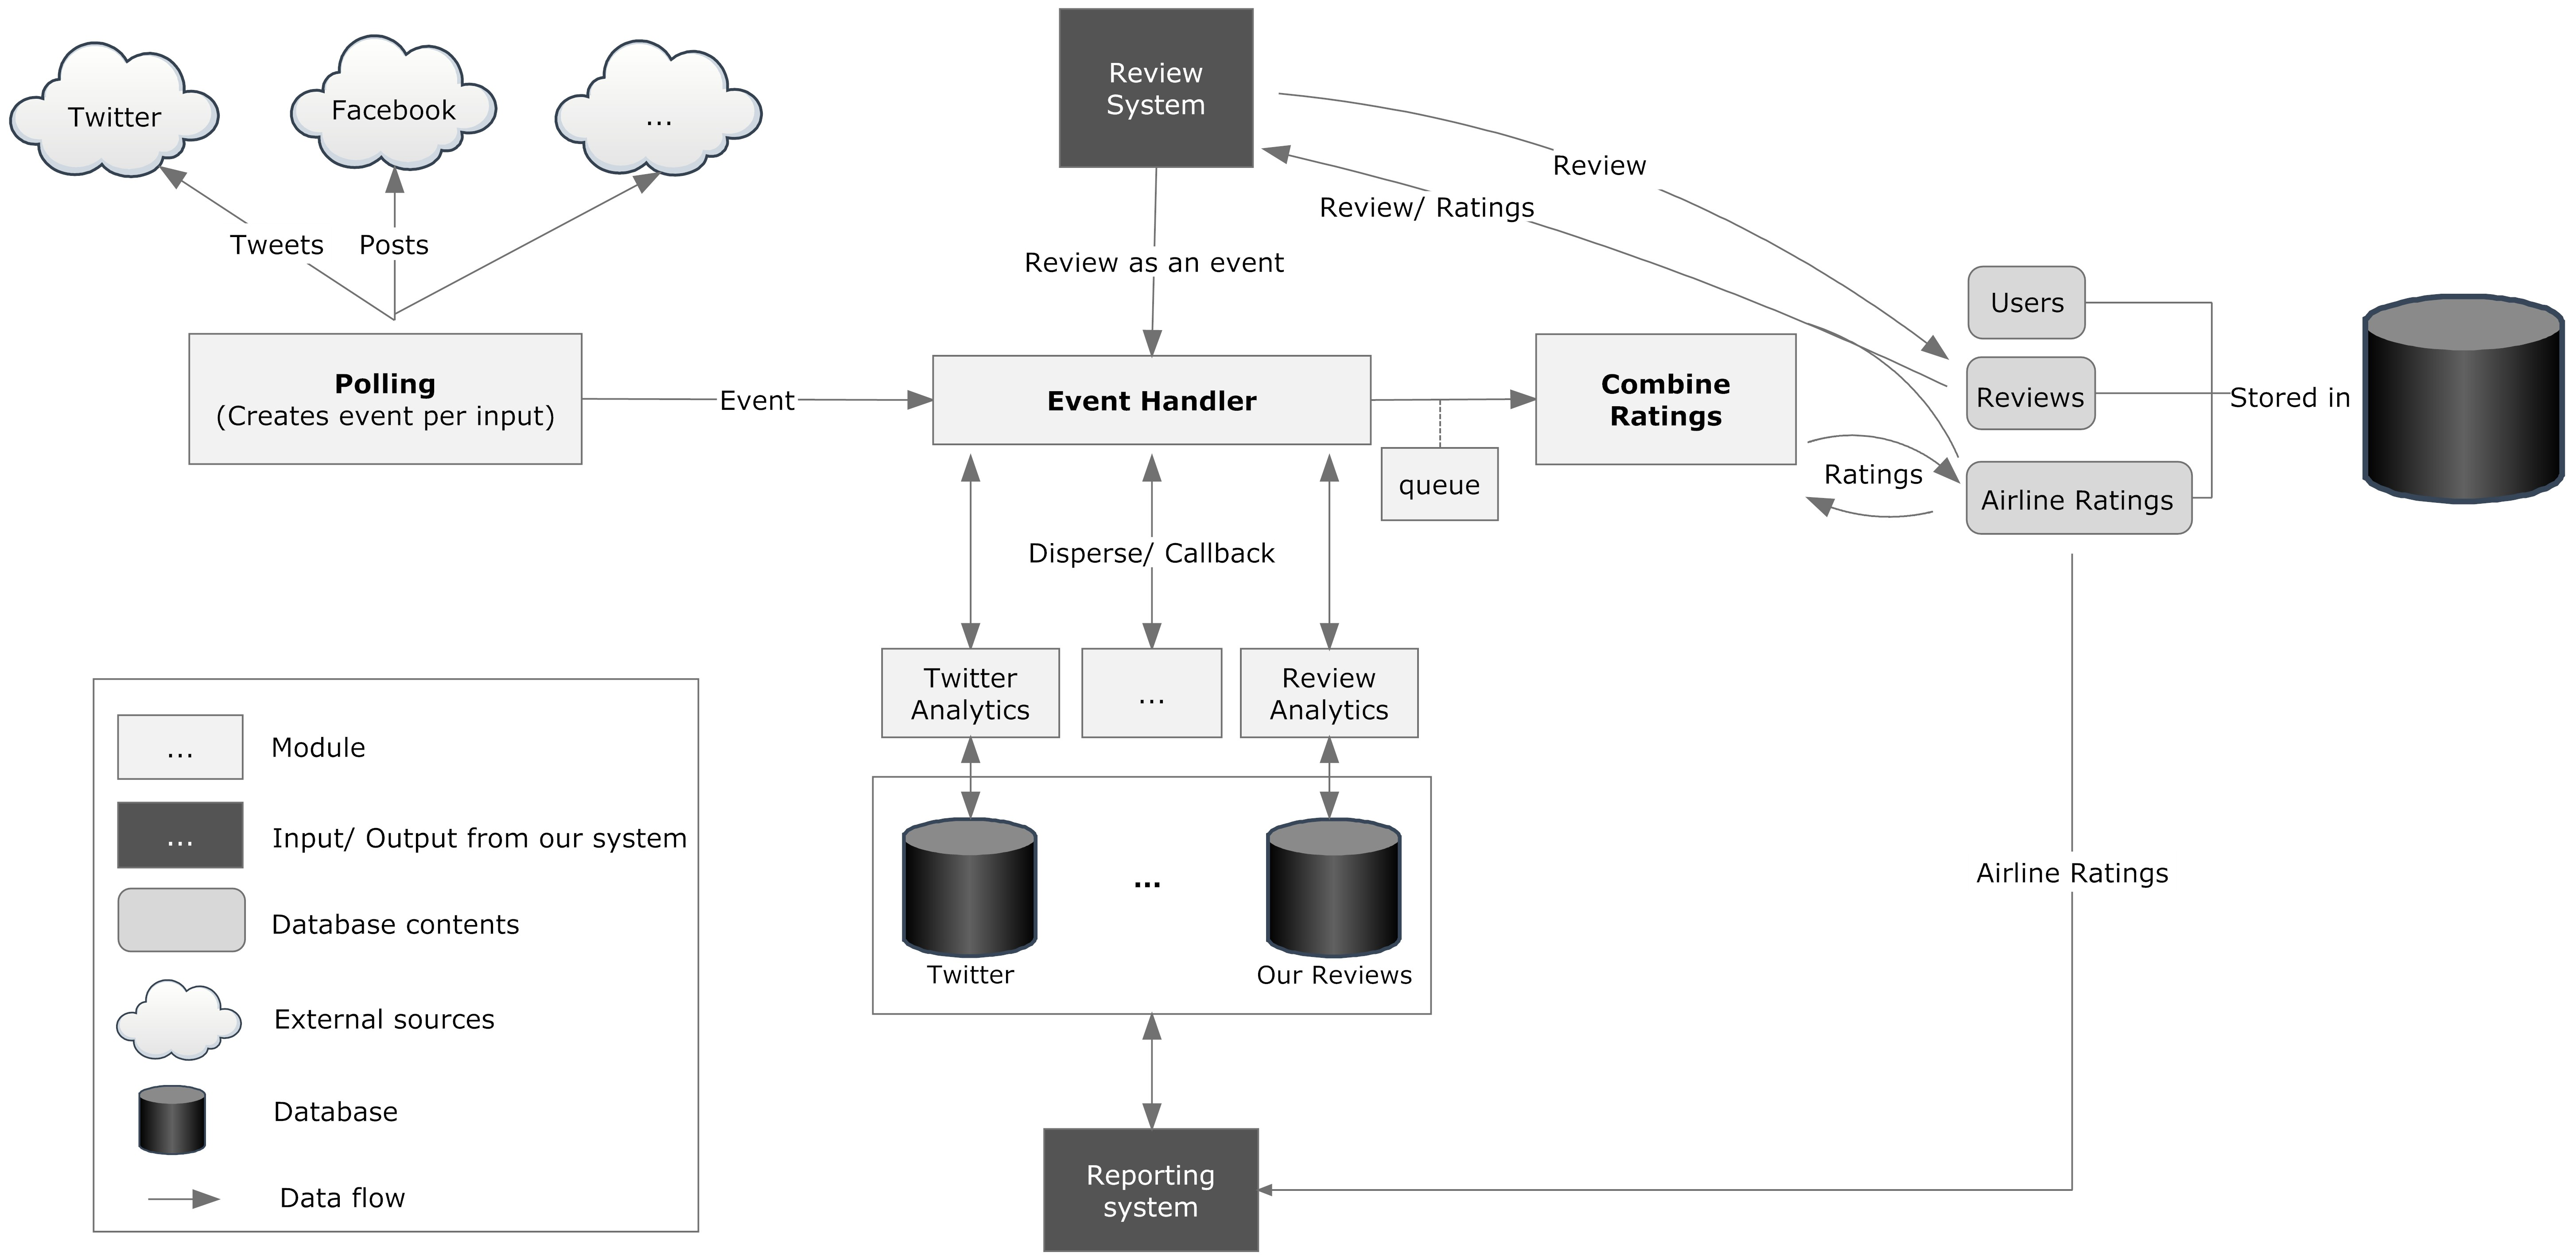
\includegraphics[width=600px]{DataFlowGraph}
\caption{Data Flow Viewpoint}
\label{fig:Data Flow}
\end{figure}
\end{landscape}

This Data Flow viewpoint \ref{fig:Data Flow} illustrates the flow of data within the back-end of the system. In this picture the review and reporting system are shown as black boxes to illustrate that their functionality is of no importance in this picture.
In the related design decisions it was argued that combining the rating with incremental updates was best for performance and scalability. Note that in the flow only the back-end of the system is given, because of the importance of handling the large data sets. Each of the modules and arrows in the viewpoint are explained here after.

\subsubsection{Polling}
The polling module is responsible for obtaining reviews from external data sources. It polls every external source on a given time-frame which is different for each external source. The reviews are not formatted and there original data format from the external source is kept. The rationale behind this decision is that all the reviews from external sources are significantly different of each other. Parsing them into a general format would lead to data loss or lots of undefined fields. The decision is further elaborated in the appendix at \ref{dd:save-raw}. The unformatted reviews are then passed on to the event handler as events. An event is defined as a single unformatted review either from external or internal sources.

\subsubsection{Event handler}
The event handler receives the events from both the polling module (external sources) and the review system (internal source). The responsibility of the event handler is to send these events to the analytics module specific to that data source. The event handler allows for parallel processing of reviews and greatly increased the performance and scalability compared to a more traditional pipeline model. This decision is further elaborated on in the appendix at \ref{dd:large-data}.

\subsubsection{Analytics}
Each data source has its own analytics module, because the data must be treated differently from external sources as they are of different format. The separate analytics modules have the added benefit of allowing for meta-analysis specific to a given data source. An example could be the amount of followers on twitter.

The analytics module analyses the unformatted review and produces a rating on a given scale for a certain or multiple categories (Overall, food, timeliness etc.). The unformatted review together with the analysed ratings are then stored in the analytics database of the data source. This is a requirement by the Initiator and KLM. The decision is further discussed in the appendix \ref{dd:data-format}. The ratings are also send of the combine ratings module in order to update the rating of the airline that is related to the review.

\subsubsection{Combine Ratings}
The combine ratings module is responsible for combining the ratings from the individual reviews into a final rating for an airline. The module receives the ratings from the analytics module and obtains the old rating from the main database. These two are combined in order to form a new rating. The process of iteratively combining ratings instead of recalculating is made for performance reasons as it is much cheaper and efficient to not recalculate the ratings that are already in the final rating of the airline. This decision is discussed in the appendix at \ref{dd:recalc-comb}. The ratings are based on an airline and a specific category (overall, timeliness, food etc.).

\subsubsection{Modules}
The functionality of each of the modules is discussed in the functional view. Hence in this section only the data flow regarding each of the modules is discussed:

\begin{enumerate}
\item \emph{R \& R module} A new review is inserted as event into the event handler which can pass it off to the specific analytics module. The decision was made to save the internal reviews twice: once in the main database and once when the they are analysed in the Analytics database. This allows the users to see the reviews without accessing the analytics database, but increases overhead as the same data is almost saved twice.
\item \emph{Reporting module} The reporting module retrieves information from the analytics database which contain all the analysed data together with the raw reviews. It must also be able to access the main database for the latest final ratings.
\item \emph{Authentication module} The user data for logging purposes is saved in the main database. The data contains sensitive information and is therefore encrypted.
\item \emph{Billing module} In order to make a profit airlines need to pay for their functionality. Therefore the billing module is able to read the current enlisted airlines and write to the database if the airlines have paid or not.
\item \emph{Messaging module} The messages are saved separately in the main database. Because they can contain user sensitive information (e.g. Flight numbers, names) the whole messages are saved in an encrypted form.
\end{enumerate}

% % % \input{DataFlow}

\subsection{Data Flow Viewpoint}

\begin{itemize}
\item Related stakeholders: KLM, Initiator
\item Related Concerns: Data Integrity, Performance, Scalability
\item Related design decisions: How is the data split up into multiple databases?; How do we handle large data-sets?; Recalculate or Combine rating?; Incremental or Time-interval update?; Flight-Information
\end{itemize}

\newpage
\begin{landscape}
\begin{figure}
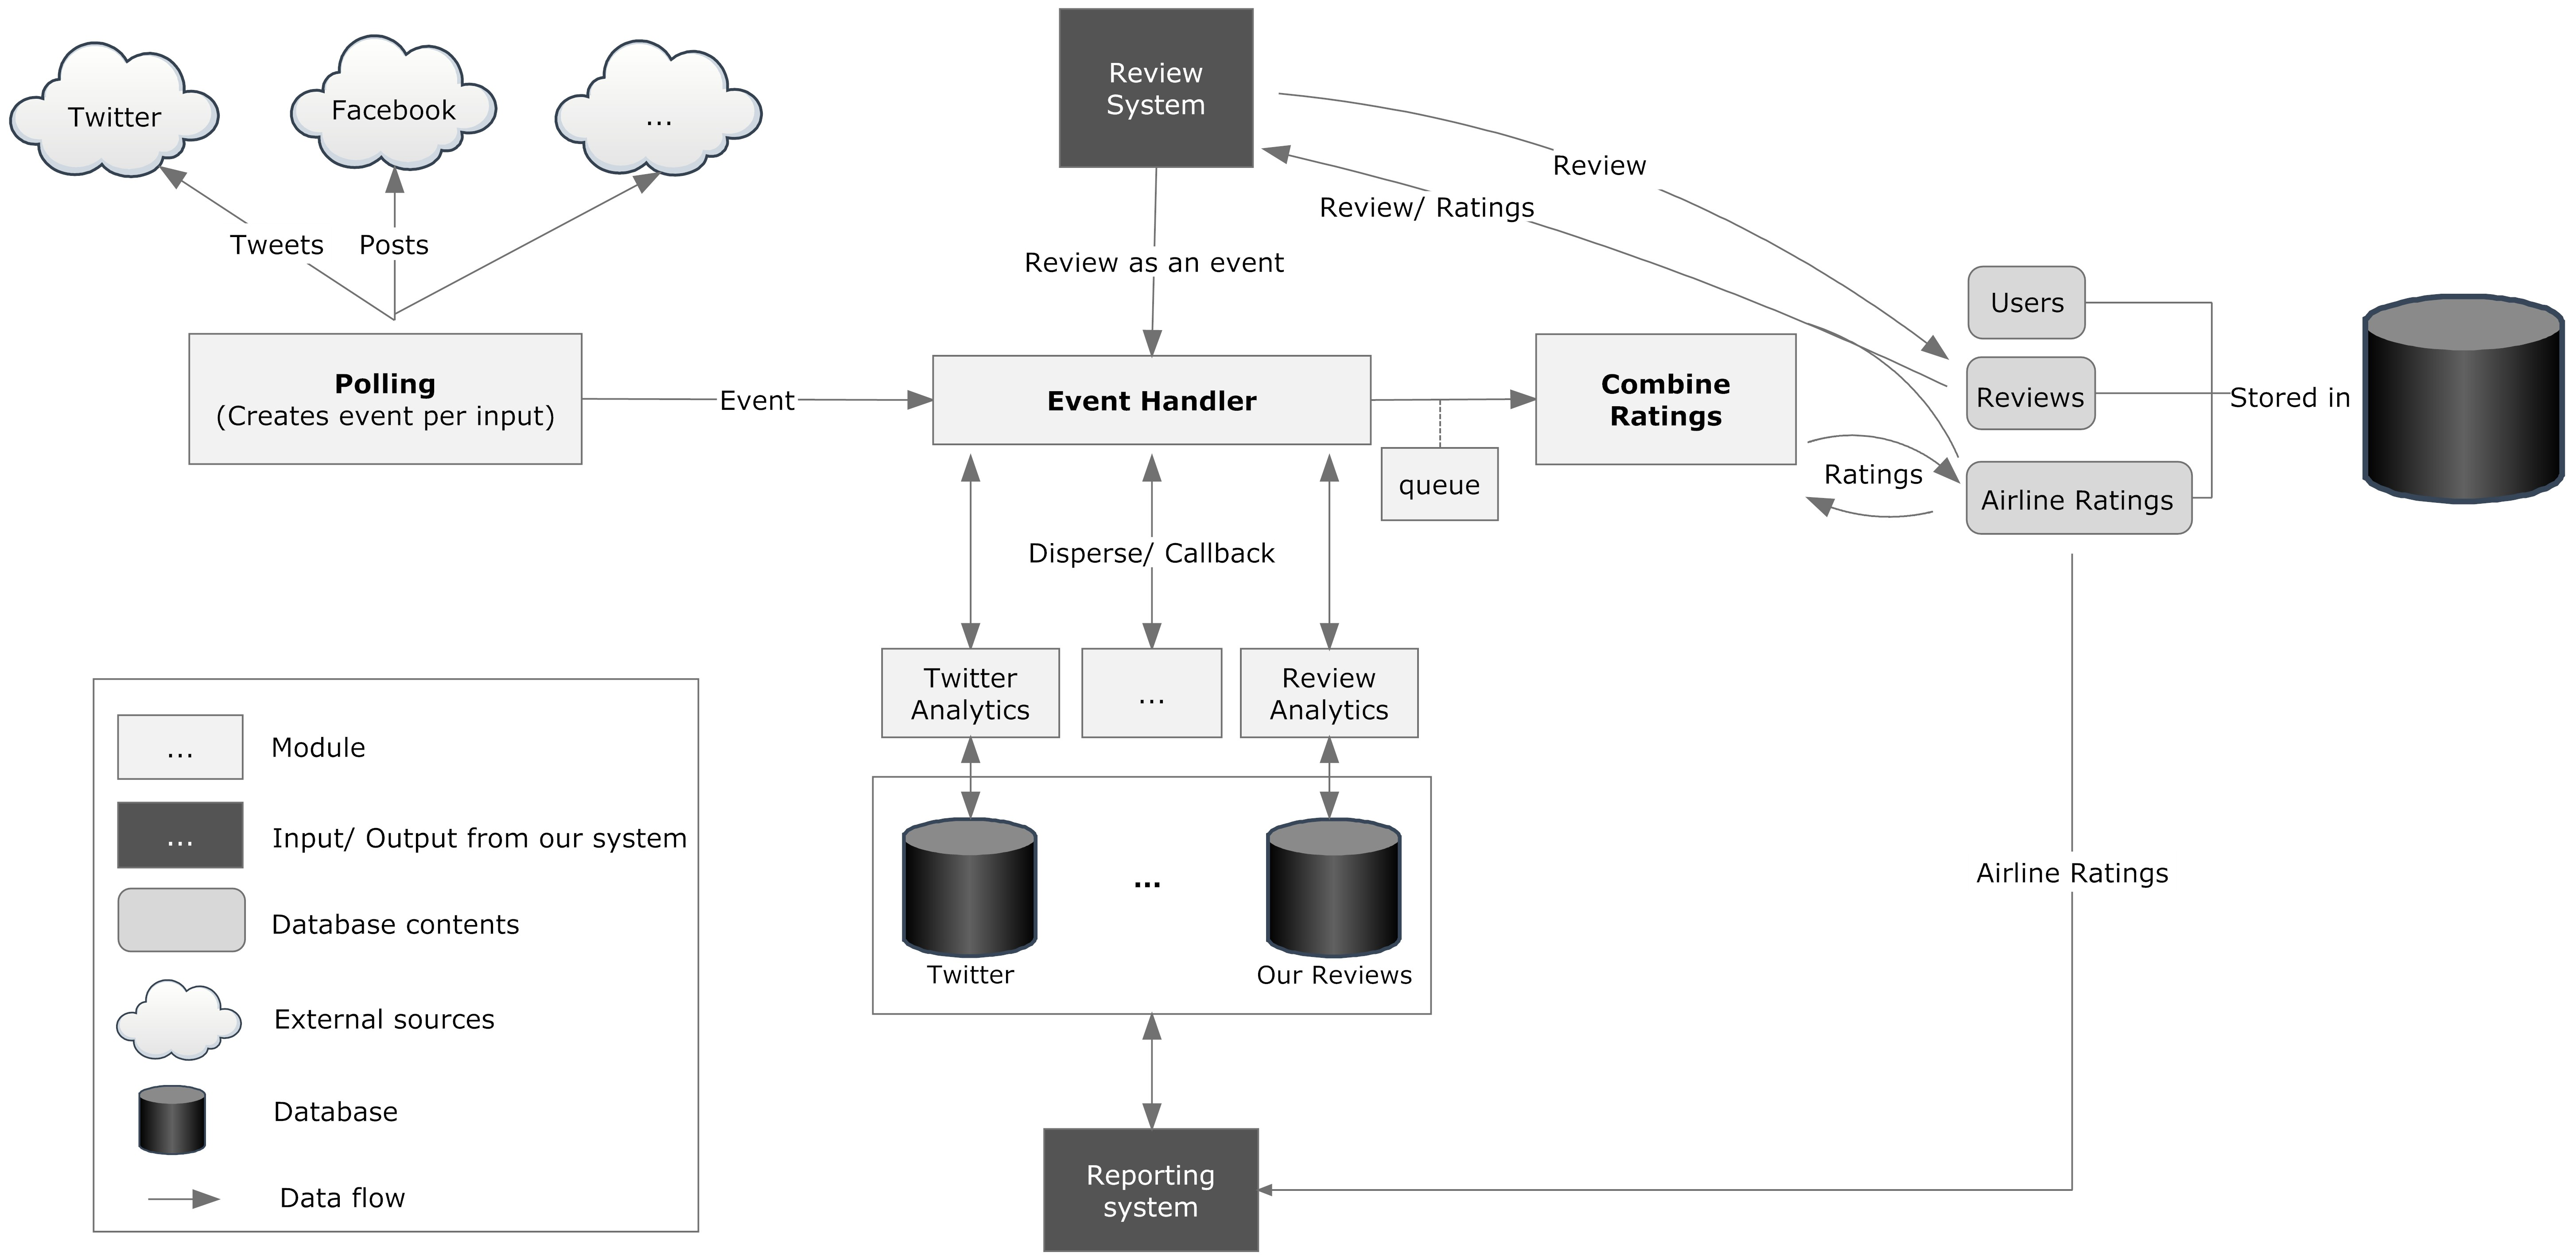
\includegraphics[width=600px]{DataFlowGraph}
\caption{Data Flow Viewpoint}
\label{fig:Data Flow}
\end{figure}
\end{landscape}

This Data Flow viewpoint \ref{fig:Data Flow} illustrates the flow of data within the back-end of the system. In this picture the review and reporting system are shown as black boxes to illustrate that their functionality is of no importance in this picture.
In the related design decisions it was argued that combining the rating with incremental updates was best for performance and scalability. Note that in the flow only the back-end of the system is given, because of the importance of handling the large data sets. Each of the modules and arrows in the viewpoint are explained here after.

\subsubsection{Polling}
The polling module is responsible for obtaining reviews from external data sources. It polls every external source on a given time-frame which is different for each external source. The reviews are not formatted and there original data format from the external source is kept. The rationale behind this decision is that all the reviews from external sources are significantly different of each other. Parsing them into a general format would lead to data loss or lots of undefined fields. The decision is further elaborated in the appendix at \ref{dd:save-raw}. The unformatted reviews are then passed on to the event handler as events. An event is defined as a single unformatted review either from external or internal sources.

\subsubsection{Event handler}
The event handler receives the events from both the polling module (external sources) and the review system (internal source). The responsibility of the event handler is to send these events to the analytics module specific to that data source. The event handler allows for parallel processing of reviews and greatly increased the performance and scalability compared to a more traditional pipeline model. This decision is further elaborated on in the appendix at \ref{dd:large-data}.

\subsubsection{Analytics}
Each data source has its own analytics module, because the data must be treated differently from external sources as they are of different format. The separate analytics modules have the added benefit of allowing for meta-analysis specific to a given data source. An example could be the amount of followers on twitter.

The analytics module analyses the unformatted review and produces a rating on a given scale for a certain or multiple categories (Overall, food, timeliness etc.). The unformatted review together with the analysed ratings are then stored in the analytics database of the data source. This is a requirement by the Initiator and KLM. The decision is further discussed in the appendix \ref{dd:data-format}. The ratings are also send of the combine ratings module in order to update the rating of the airline that is related to the review.

\subsubsection{Combine Ratings}
The combine ratings module is responsible for combining the ratings from the individual reviews into a final rating for an airline. The module receives the ratings from the analytics module and obtains the old rating from the main database. These two are combined in order to form a new rating. The process of iteratively combining ratings instead of recalculating is made for performance reasons as it is much cheaper and efficient to not recalculate the ratings that are already in the final rating of the airline. This decision is discussed in the appendix at \ref{dd:recalc-comb}. The ratings are based on an airline and a specific category (overall, timeliness, food etc.).

\subsubsection{Modules}
The functionality of each of the modules is discussed in the functional view. Hence in this section only the data flow regarding each of the modules is discussed:

\begin{enumerate}
\item \emph{R \& R module} A new review is inserted as event into the event handler which can pass it off to the specific analytics module. The decision was made to save the internal reviews twice: once in the main database and once when the they are analysed in the Analytics database. This allows the users to see the reviews without accessing the analytics database, but increases overhead as the same data is almost saved twice.
\item \emph{Reporting module} The reporting module retrieves information from the analytics database which contain all the analysed data together with the raw reviews. It must also be able to access the main database for the latest final ratings.
\item \emph{Authentication module} The user data for logging purposes is saved in the main database. The data contains sensitive information and is therefore encrypted.
\item \emph{Billing module} In order to make a profit airlines need to pay for their functionality. Therefore the billing module is able to read the current enlisted airlines and write to the database if the airlines have paid or not.
\item \emph{Messaging module} The messages are saved separately in the main database. Because they can contain user sensitive information (e.g. Flight numbers, names) the whole messages are saved in an encrypted form.
\end{enumerate}


\subsection{Data Flow Viewpoint}

\begin{itemize}
\item Related stakeholders: KLM, Initiator
\item Related Concerns: Data Integrity, Performance, Scalability
\item Related design decisions: How is the data split up into multiple databases?; How do we handle large data-sets?; Recalculate or Combine rating?; Incremental or Time-interval update?; Flight-Information
\end{itemize}

\newpage
\begin{landscape}
\begin{figure}
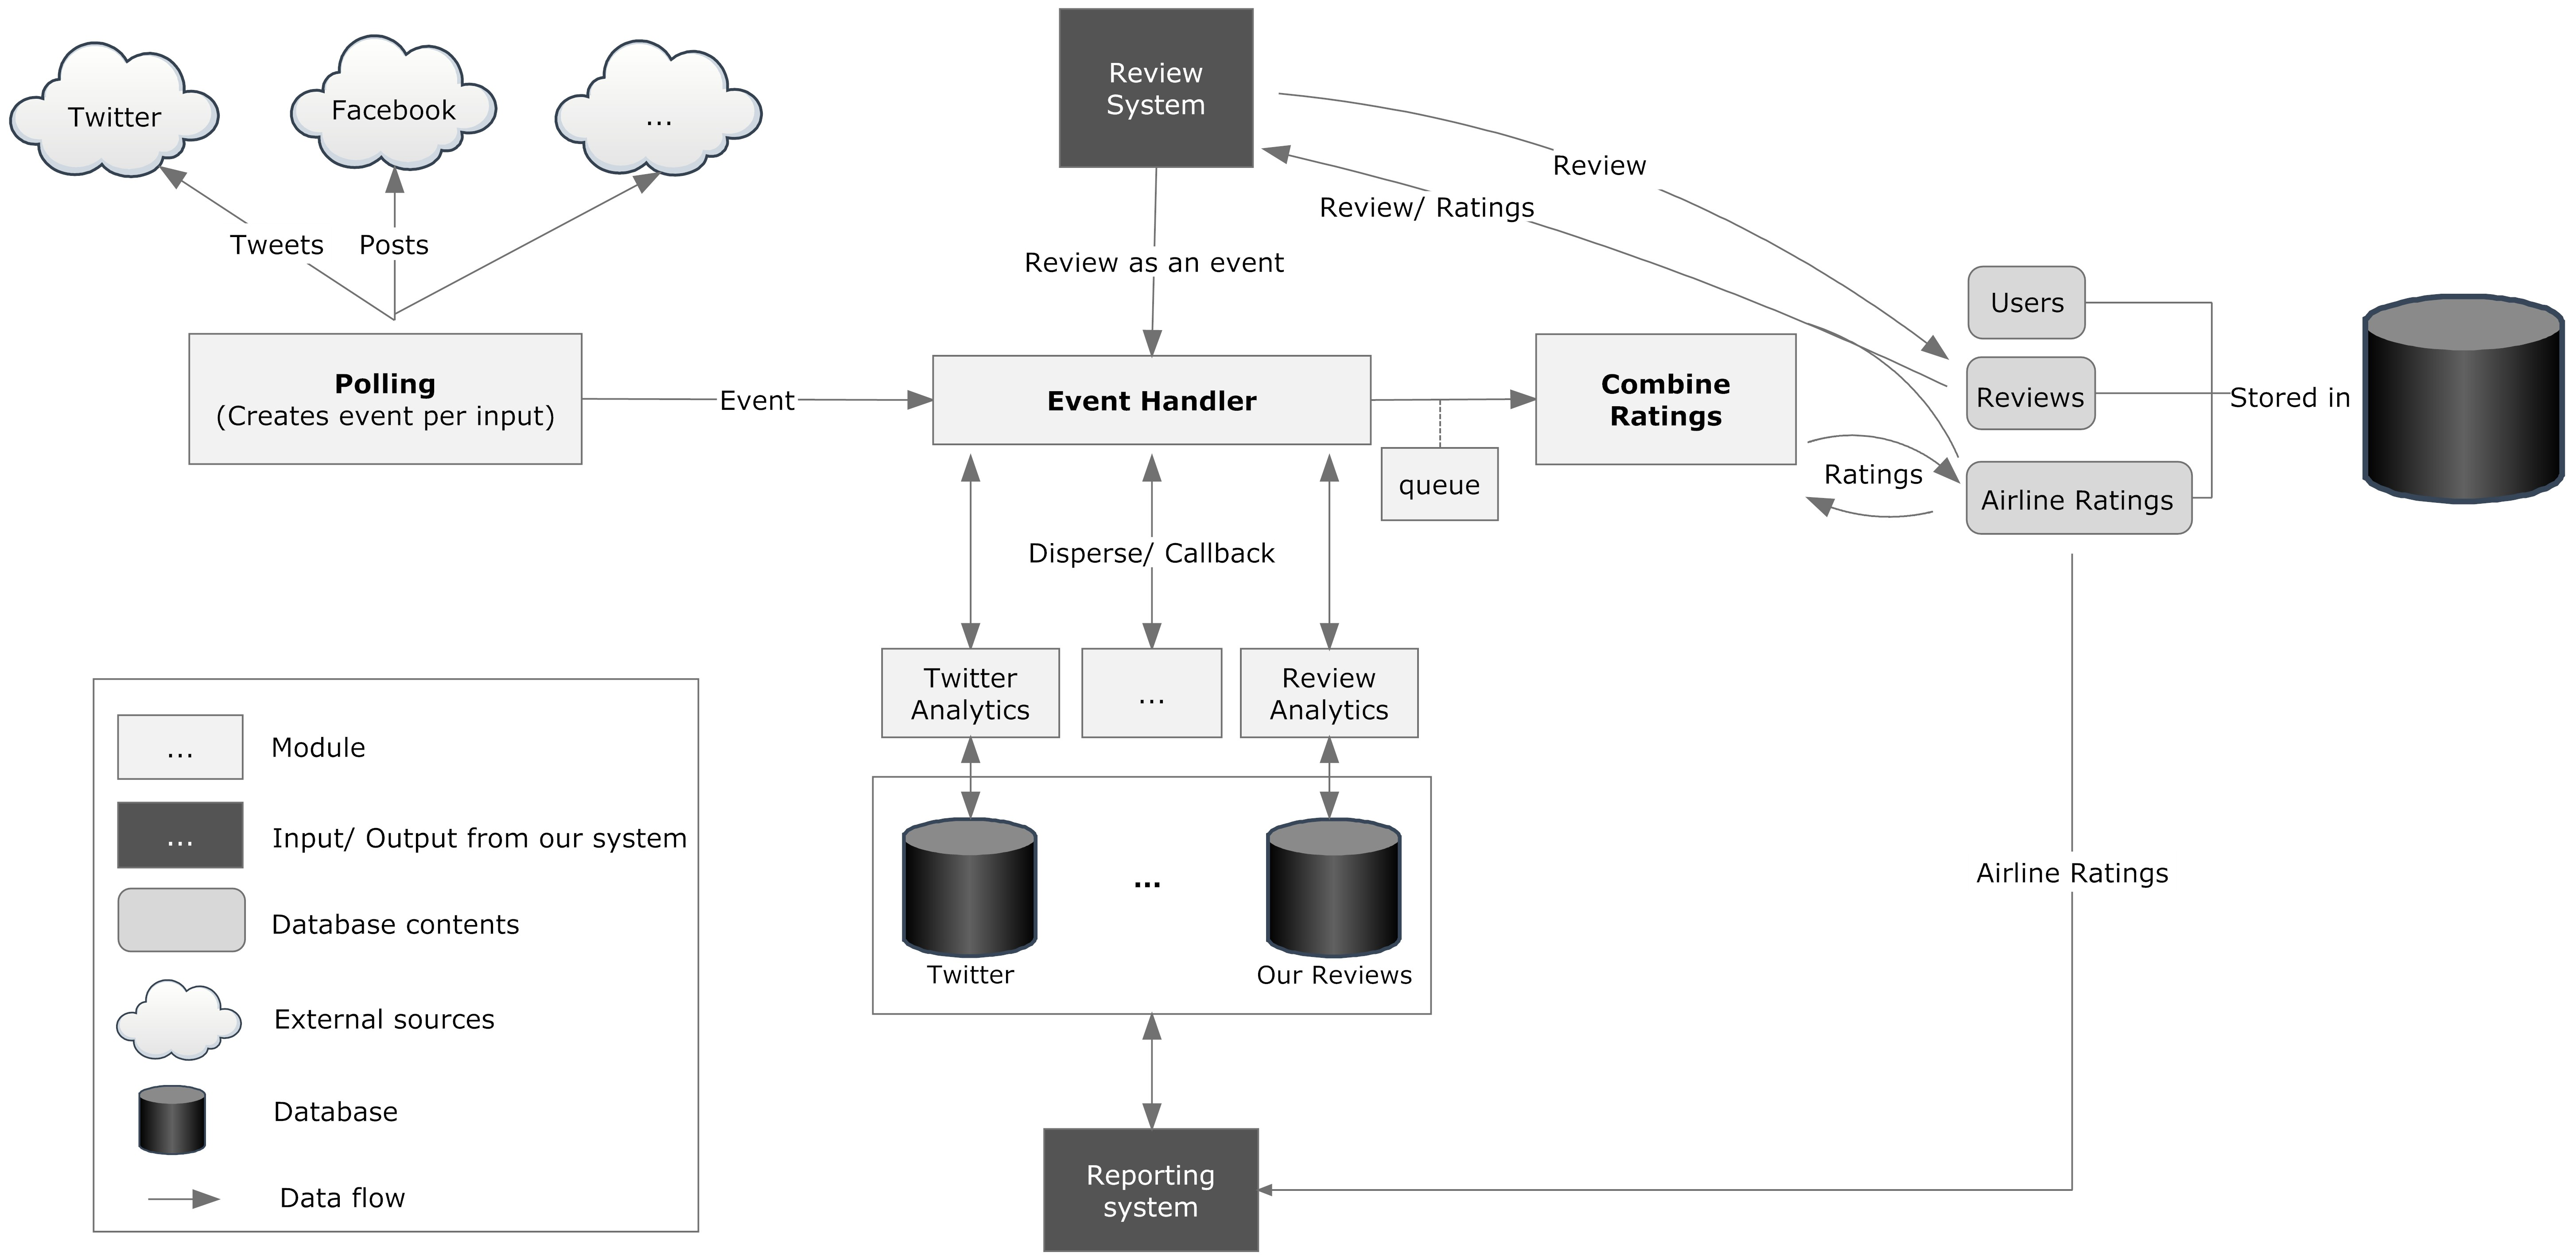
\includegraphics[width=600px]{DataFlowGraph}
\caption{Data Flow Viewpoint}
\label{fig:Data Flow}
\end{figure}
\end{landscape}

This Data Flow viewpoint \ref{fig:Data Flow} illustrates the flow of data within the back-end of the system. In this picture the review and reporting system are shown as black boxes to illustrate that their functionality is of no importance in this picture.
In the related design decisions it was argued that combining the rating with incremental updates was best for performance and scalability. Note that in the flow only the back-end of the system is given, because of the importance of handling the large data sets. Each of the modules and arrows in the viewpoint are explained here after.

\subsubsection{Polling}
The polling module is responsible for obtaining reviews from external data sources. It polls every external source on a given time-frame which is different for each external source. The reviews are not formatted and there original data format from the external source is kept. The rationale behind this decision is that all the reviews from external sources are significantly different of each other. Parsing them into a general format would lead to data loss or lots of undefined fields. The decision is further elaborated in the appendix at \ref{dd:save-raw}. The unformatted reviews are then passed on to the event handler as events. An event is defined as a single unformatted review either from external or internal sources.

\subsubsection{Event handler}
The event handler receives the events from both the polling module (external sources) and the review system (internal source). The responsibility of the event handler is to send these events to the analytics module specific to that data source. The event handler allows for parallel processing of reviews and greatly increased the performance and scalability compared to a more traditional pipeline model. This decision is further elaborated on in the appendix at \ref{dd:large-data}.

\subsubsection{Analytics}
Each data source has its own analytics module, because the data must be treated differently from external sources as they are of different format. The separate analytics modules have the added benefit of allowing for meta-analysis specific to a given data source. An example could be the amount of followers on twitter.

The analytics module analyses the unformatted review and produces a rating on a given scale for a certain or multiple categories (Overall, food, timeliness etc.). The unformatted review together with the analysed ratings are then stored in the analytics database of the data source. This is a requirement by the Initiator and KLM. The decision is further discussed in the appendix \ref{dd:data-format}. The ratings are also send of the combine ratings module in order to update the rating of the airline that is related to the review.

\subsubsection{Combine Ratings}
The combine ratings module is responsible for combining the ratings from the individual reviews into a final rating for an airline. The module receives the ratings from the analytics module and obtains the old rating from the main database. These two are combined in order to form a new rating. The process of iteratively combining ratings instead of recalculating is made for performance reasons as it is much cheaper and efficient to not recalculate the ratings that are already in the final rating of the airline. This decision is discussed in the appendix at \ref{dd:recalc-comb}. The ratings are based on an airline and a specific category (overall, timeliness, food etc.).

\subsubsection{Modules}
The functionality of each of the modules is discussed in the functional view. Hence in this section only the data flow regarding each of the modules is discussed:

\begin{enumerate}
\item \emph{R \& R module} A new review is inserted as event into the event handler which can pass it off to the specific analytics module. The decision was made to save the internal reviews twice: once in the main database and once when the they are analysed in the Analytics database. This allows the users to see the reviews without accessing the analytics database, but increases overhead as the same data is almost saved twice.
\item \emph{Reporting module} The reporting module retrieves information from the analytics database which contain all the analysed data together with the raw reviews. It must also be able to access the main database for the latest final ratings.
\item \emph{Authentication module} The user data for logging purposes is saved in the main database. The data contains sensitive information and is therefore encrypted.
\item \emph{Billing module} In order to make a profit airlines need to pay for their functionality. Therefore the billing module is able to read the current enlisted airlines and write to the database if the airlines have paid or not.
\item \emph{Messaging module} The messages are saved separately in the main database. Because they can contain user sensitive information (e.g. Flight numbers, names) the whole messages are saved in an encrypted form.
\end{enumerate}


\subsection{Concurrency Viewpoint}

\begin{itemize}
\item Related stakeholders: KLM, Initiator
\item Related Concerns: Availability, Performance, GreenIT
\item Related design decisions: Redudancy; Concurrency
\end{itemize}

\newpage
\begin{landscape}
\begin{figure}
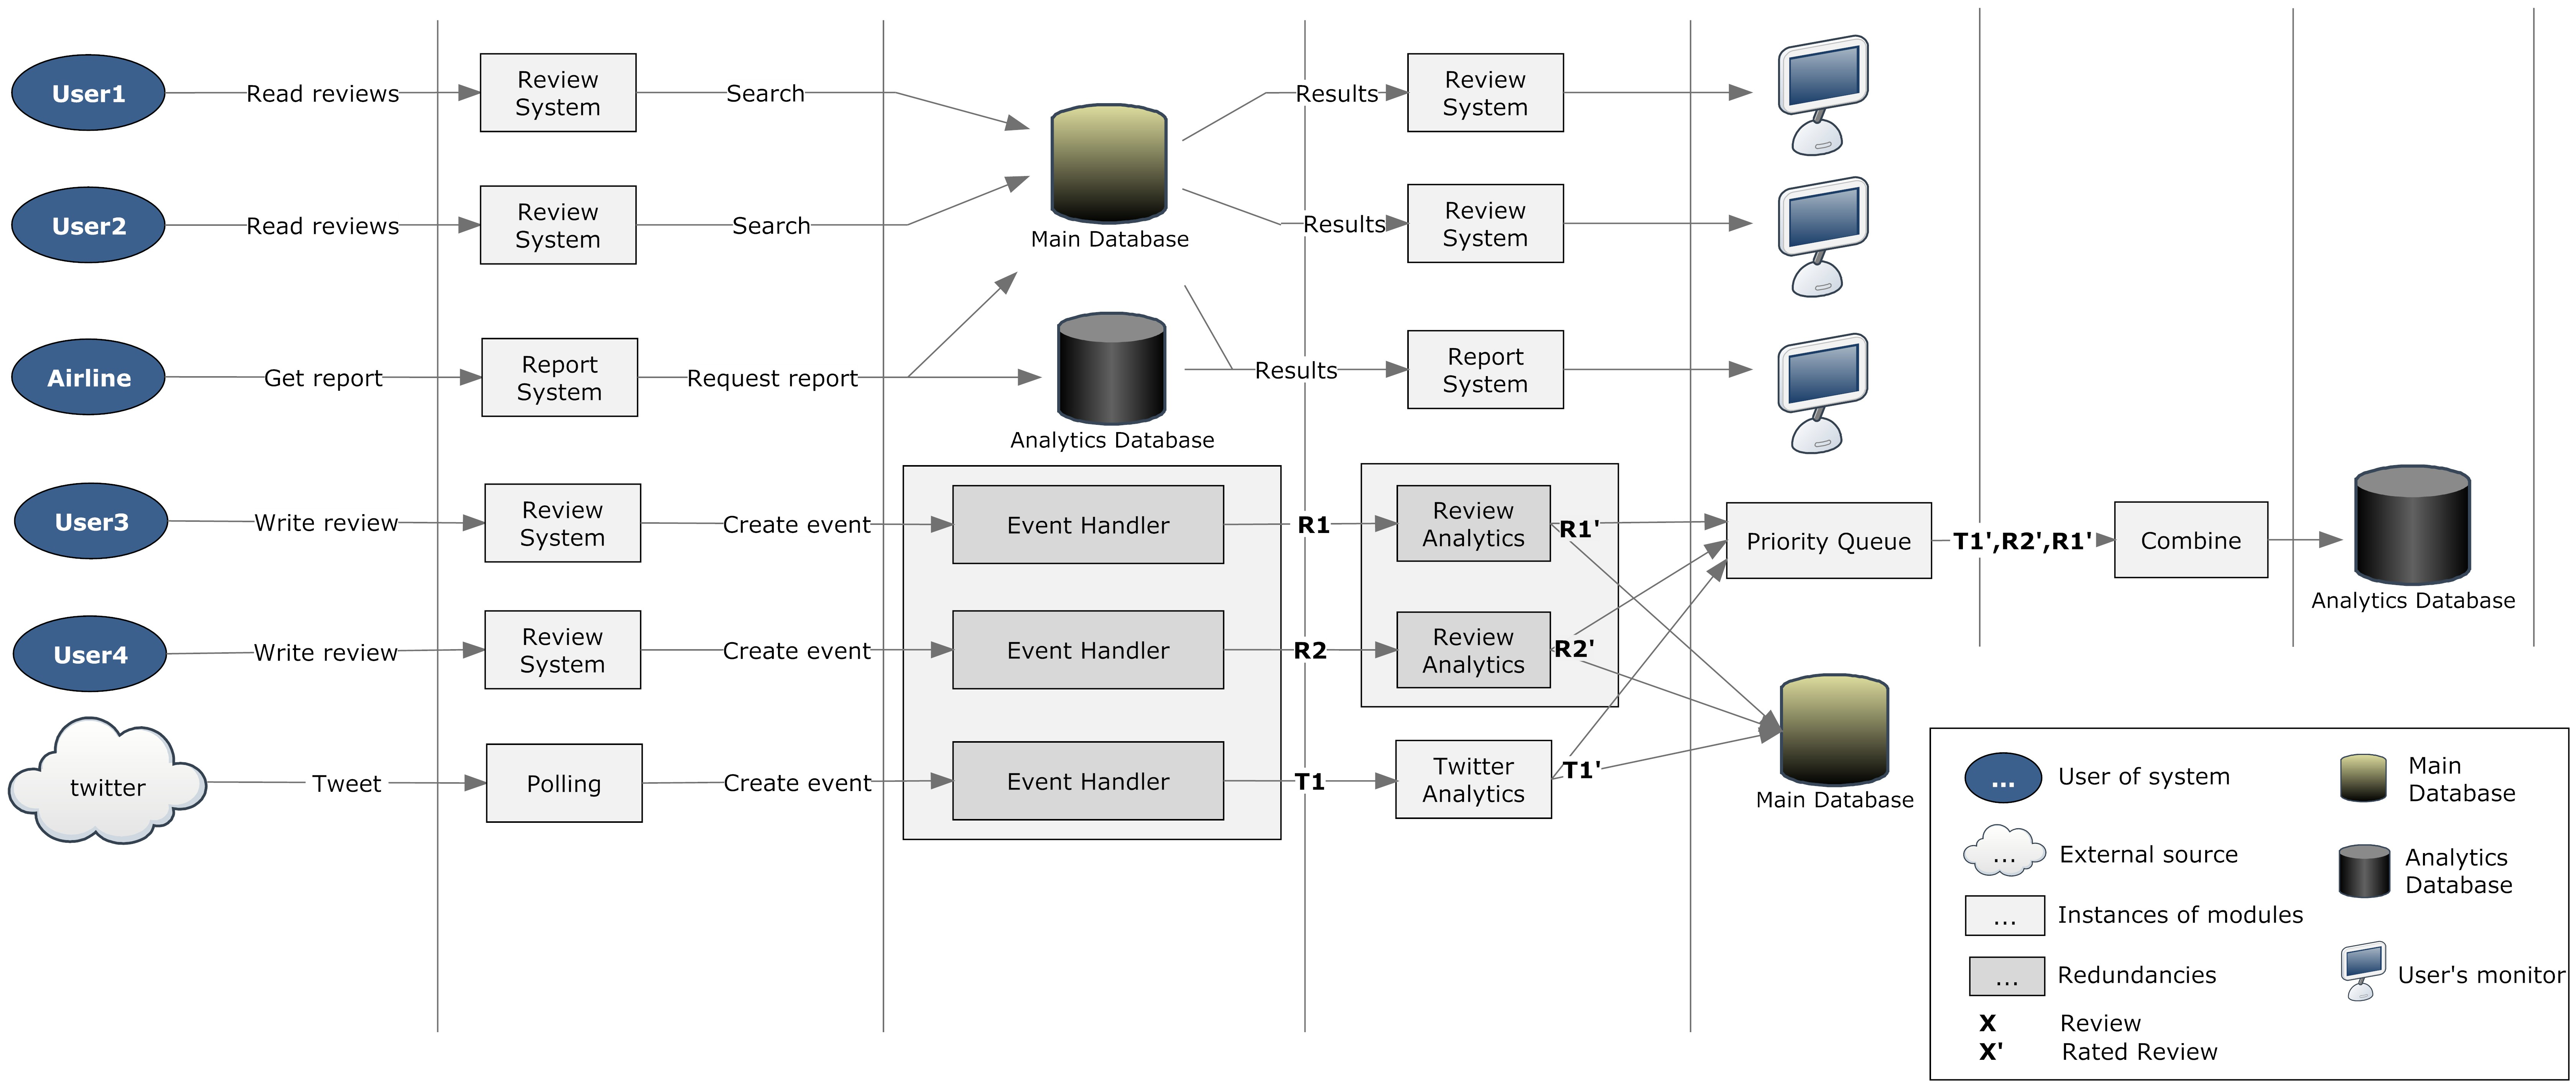
\includegraphics[width=600px]{ConcurrencyViewpoint.jpg}
\caption{Concurrency Viewpoint}
\label{fig:concurrency}
\end{figure}
\end{landscape}

The concurrency viewpoint (see fig.~\ref{fig:concurrency}) illustrates how the system behaves when different users perform different operations on it.the flow of data within the back-end of the system. In this figure the registered users or guests that search or read reviews are represented by the Users Reading element and the registered users that write a  review are represented as Users Writing. This separation is necessary because these operations are handled differently by the system since the writing operation changes the state of the database while the reading operation does not. The airlines are represented only by one entity because there is no need to separate the search or the statistics results since they are both reading operations and do not cause any change on the database's state. Finally, to represent the external sources we do not need to separate them since they are handled the same way by the system.

In the related design decisions it is discussed that redundancy will increase availability by eliminating single points of failure. Although it may decrease performance, it makes FlyWithUs a more robust system. 

\subsubsection{Instances of Modules}

A module's instances are separate processes that perform the same operations. For example, different instances of R\&R module respond to the users' requests, these instances can be different processes run on web servers. Additionally, instances of the modules review analytics and an external source analytics (eg. Facebook, Twitter, trip Advisor etc.) can run concurrently as different threads since the process of each post is dealt independently.

\subsubsection{Redundancies}

This viewpoint also puts forth single points of failure such as the event handler, the queue and the combine module. If any of these modules fails the system will have to revert to a previous state losing some the data collected. To avoid that, the system can have redundant modules that perform the same functionality and are synchronized, if any of them fails the others can continue from the point of failure without losing any data. Although it will increase the cost and will have negative impact on green IT, the stakeholders insisted on not losing any data and make the system as available as possible.


%Appendixes go here
\appendix

\section{Requirements}
This Appendix describes the functional and non-functional requirements given by the stakeholders in different meetings. The stakeholders ,with the abbreviation used in this appendix, involved with these requirements are: the initiator (Init), the Dutch government (Dg), EU-Claim (EUC) and AirFrance-KLM (KLM). 

\subsection*{Functional Requirements}
The functional requirements are given in prioritization order, the first requirement being the most important. 

\begin{longtable}{| p{10cm}| l | l |}
\hline
\textbf{Requirement} & \textbf{Abbreviation} & \textbf{Related stakeholder} \\ \hline
Show the ratings and reviews of all airlines to all users & Show ratings & Init \\ \hline
Post, read, vote and search reviews including ratings & Post/Read/Search & Init \\ \hline
A messaging system where airlines can get in touch with customers & Messaging & Init, KLM \\ \hline
Collect data from external sources like twitter and tripadvisor & Data gathering & Init, KLM \\ \hline
Combine the data from external sources to an airline rating & Data combining & Init, KLM \\ \hline
A reporting tool & Reporting & KLM \\ \hline
A transparent and fair way to calculate the airline ratings & Transparency & EUC \\ \hline
Store the (raw) external data & Save & Init \\ \hline
The system should be able to keep track of the B2B users for offline payment & Billing & Init \\ \hline
Provide flight information to influence the weight of a review & Flight Information & KLM \\ \hline
The ability to see the statistics of other airlines if permission is granted & Statistics & KLM \\ \hline 
% Airlines cannot statistics about each other if permission is not granted

\end{longtable}

\subsection*{Non-functional Requirements}
The non-functional requirements are given in prioritization order, the first requirement being the most important. 

\begin{longtable}{| p{10cm}| l | l |}
\hline
\textbf{Requirement} & \textbf{Abbreviation} & \textbf{Related stakeholder} \\ \hline
The system should give the data within two seconds & Performance & Init, KLM \\ \hline
The user data should only be available for the user itself and not for the public. & Privacy & Dg, EUC \\ \hline
Scalability is needed for both the users and the amount of reviews.& Scalability & Init \\ \hline
External data-sources should be addable without affecting the rest of the system & Adding data-sources & Init \\ \hline
The server needs to be hosted in the Netherlands & Hosting & Dg, EUC \\ \hline
The project should be a GreenIT project & GreenIT & Dg \\ \hline
\end{longtable}


\clearpage
\section{Formal Design Decisions}
This appendix states the design decisions that were taken during the process of designing an architecture. Figure \ref{fig:ddtree} shows the tree of the design decisions that will each be further elaborated on this section.

\begin{figure}[!ht]
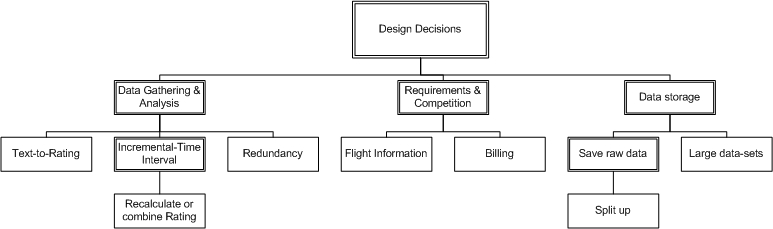
\includegraphics[width= 410px]{DDTree}
\caption{The design decision tree}
\label{fig:ddtree}
\end{figure}

%The Design Decisions
\setcounter{table}{0}

\clearpage

{\large\captionof{table}{Data format}}
\begin{tabular}{ l  p{10cm}}
\hline
\bf Issue & The external sources have a unique format related to them. The system needs to be able to combine all these reviews into a final rating of a generalized format. How will we deal with the unique format of the external sources?\\
\hline
\bf Decision & The unique format is kept in before it is analyzed. The analyzing step converts the unique format into a rating on a category (e.g. food, timeliness) which the system can use and combine \\
\hline
\bf Status & Decided\\
\hline
\bf Group & Analysis of data; \\
\hline
\bf Assumptions & The data from external sources cannot easily be combined because they all have a significantly different format.  \\
\hline
\bf Constraints & None \\
\hline
\bf Positions & Keep the unique format before analyzing the data. \newline\newline
Parse the unique format from external sources into a general format the analyses module can use. 
 \\
\hline
\bf Argument & The external sources contain different layouts parsing them into a general format would either lead to data loss or lot of ‘undefined’ fields. However the analyses module does not need to account for different kinds of data which decreases its complexity. The potential loss of data (and maybe meta-data)  would however decrease the effectiveness of the analyses module. Therefore the decision was made to keep and store the data in a unique format.  \\
\hline
\bf Implications & The storage system needs to be able to handle the data from external sources. The analysis module needs to handle multiple lay-outs of the external sources.  \\
\hline
\bf Related decisions & \\
\hline
\bf Related requirements  & Data combining, Data Storage \\
\hline
\end{tabular}

\newpage

\label{dd:flight-inf}
\captionof{table}{Flight Information}
\begin{tabular}{ l  p{10cm}}
\hline
\bf Issue & It may occur that a flight is delayed due to external factors outside of the airlines responsibilities (e.g. weather). A bad review may affect the airlines rating which may not be considered a desirable effect. Do we want Flight Information to influence the rating of an airline or shall we not regard it. \\
\hline
\bf Decision & The status is still pending awaiting conversation with the involved stakeholders. \\
\hline
\bf Status & Pending \\
\hline
\bf Group & Analysis of data; \\
\hline
\bf Assumptions & Users will write reviews even if factors are outside of the airlines responsibilities. \\
\hline
\bf Constraints & None \\
\hline
\bf Positions & Cross-match flight information from airlines into the rating algorithm to avoid the influence of those reviews towards the rating \newline\newline
Let the airlines search for reviews based on flight information, but not change the rating algorithms. \newline\newline
Leave the problem out the scope of the system. \\
\hline
\bf Argument & If airlines can influence the rating algorithms than this greatly decreases the transparency of the system. This problem applies to each airline so it does not decrease the fairness of the system. The second option gives airlines the ability to spot the influence of those bad reviews, but not alter their influence. This keeps the system transparent. \\
\hline
\bf Implications &The implications are given after the decision is taken. \\
\hline
\bf Related decisions & Split-up \\
\hline
\bf Related requirements  & Flight information, Transparancy \\
\hline
\end{tabular}

%\newpage
%
\captionof{table}{Interfaces}
\begin{tabular}{ l  p{10cm}}
\hline
\bf Issue & The airlines and customers use different services on the system as a result they will have different options on their interface. This can be accomplished in two ways, either they can have entirely different interfaces or use the same lay-out. \\
\hline
\bf Decision & Two different external sites.\\
\hline
\bf Status & Pending\\
\hline
\bf Group & User Experience;  \\
\hline
\bf Assumptions & None \\
\hline
\bf Constraints & None\\
\hline
\bf Positions &  Have one website, when a user is logged in the interface changes depending on his/ her type. \newline\newline
Have two different log in pages so the airlines will never come across the regular user website and vice versa.
\\
\hline
\bf Argument & The second option is more appealing to the airlines, because they have their own unique landing page. This also limits the users knowledge of the airlines and might help any security issues related to users trying to login as airlines. \\
\hline
\bf Implications & The implications depend on the decision that remains to be taken. \\
\hline
\bf Related decisions & \\
\hline
\bf Related requirements  & \\
\hline
\end{tabular}


\newpage

\captionof{table}{How are large data-sets handled?}
\begin{tabular}{ l  p{10cm}}
\hline
\bf Issue & Data collected from external sources requires a great amount of storage over time. It also needs to be analyzed and have statistics generated/stored.\\
\hline
\bf Decision & Event type of dispatching.\\
\hline
\bf Status & Decided\\
\hline
\bf Group & Data storage \\
\hline
\bf Assumptions & The number of incoming data sets is that of a big data type.  \\
\hline
\bf Constraints & None \\
\hline
\bf Positions & Pipeline model \newline\newline
Event type of dispatching
 \\
\hline
\bf Argument & In a pipeline model each step (Storing, analyzing, Storing statistics + rating) is performed in a sequence. Every review from every external source goes through the same system pipe. This is bad for scalability reasons as more and more reviews would clog up the system. The event type of dispatching can disperse reviews through a channel depending on their source. This creates paralism in the system and is more easily scalable. By collecting the data and sending it to the analyzers, FlyWithUs can generate the rating and score before storing it all. This way there is no need to read and write twice from intermediate storage which improves performance. \\
\hline
\bf Implications & An event handler needs to be developed with clear contracts towards the other components within the system.  \\
\hline
\bf Related decisions & How is the data split up into multiple databases? \\
\hline
\bf Related requirements  & Performance, Scalability \\
\hline
\end{tabular}


%\newpage
%
\label{dd:payment}
\captionof{table}{Online Payment}
\begin{tabular}{ l  p{10cm}}
\hline
\bf Issue & The airlines should pay FlyWithUs for using the services this can be done online and offline (automatically based on contract). \\
\hline
\bf Decision & Payment will be done automatically (offline). \\
\hline
\bf Status & Decided \\
\hline
\bf Group & User Experience;  Requirements \\
\hline
\bf Assumptions & None \\
\hline
\bf Constraints & None \\
\hline
\bf Positions & Online payment via for example Ideal. \newline\newline
Automatic payment by the airline based on a contract. \\
\hline
\bf Argument & In order to support online payment the database needs to be ACID which will restrict the options for databases. The AirFrance-KLM stakeholder informed us that companies are used to paying automatically, through bank, and preferred this over using Ideal. \\
\hline
\bf Implications & No payment system needs to be developed. \\
\hline
\bf Related decisions & \\
\hline
\bf Related requirements  & \\
\hline
\end{tabular}

\newpage
\input{recalculate-or-combine}
\newpage

\label{dd:inc-or-time}
\captionof{table}{Incremental or Time-interval updates?}
\begin{tabular}{ l  p{10cm}}
\hline
\bf Issue & Updating the statistics and rating can be done when receiving new data or on a time interval. \\
\hline
\bf Decision & Updating when receiving data, utilizing a queue to spread load. \\
\hline
\bf Status & Decided \\
\hline
\bf Group & Data Analysis \\
\hline
\bf Assumptions & None \\
\hline
\bf Constraints & None \\
\hline
\bf Positions & Update statistics and rating on a time-interval. \newline \newline
Update incrementally. \\
\hline
\bf Argument & If a time-interval based system is used, the system will can create peak loads and lots of idling, which means a very variable resource usage. This in turn means that you both have a system running for nothing and that it also needs to be powerful enough to handle the load at the given time-intervals. In contrast, by using an incremental approach, the load on the system can be spread out. By doing so the system requires less resources to process the data as no load peaks will occur. \\
\hline
\bf Implications & The system will always be running and performing work. \\
\hline
\bf Related decisions & None \\
\hline
\bf Related requirements  & Performance, Scalability \\
\hline
\end{tabular}

\newpage

\captionof{table}{How is the data split up into multiple databases?}
\begin{tabular}{ l  p{10cm}}
\hline
\bf Issue & How many databases gives a good maintainable system and allows for the best performance for all the different database usages?\\
\hline
\bf Decision & Split between data-mining (external and internal reviews statistics) and website data (users, conversations , ratings)\\
\hline
\bf Status & Decided\\
\hline
\bf Group & Data Storage \\
\hline
\bf Assumptions & At the very least there is website data, data-mining data and statistical data.\\
\hline
\bf Constraints & None \\
\hline
\bf Positions & All data is contained within one large database. \newline\newline
Split between data-mining (external and internal reviews statistics) and website data (users, conversations , ratings)  \newline\newline
Split between data-mining (external reviews), statistics on (external) reviews and website data (users, conversations , ratings)
 \\
\hline
\bf Argument & Keeping all the data in one large database makes it very hard to scale and generally creates performance issues related with the amount of incoming data. 
The third option leads to a greater number of databases. However the statistics are heavily related to the reviews themselves (data mining) splitting these two up creates fragmented data. 
 \\
\hline
\bf Implications & There is a need for multiple databases that have some relation to each other. These relations need to be clearly defined in order for the system need to completely get out of synch. \\
\hline
\bf Related decisions & How do we handle large data-sets? \\
\hline
\bf Related requirements  & Data Storage, Performance, Scalability\\
\hline
\end{tabular}

\newpage
\input{text-to-rating}
\newpage

\label{dd:redundancy}
\captionof{table}{Redundancy}
\begin{tabular}{ l  p{10cm}}
\hline
\bf Issue & Single points of failure form a risk in the system. The whole system may become unavailable if these points crash or are otherwise inhibited from doing their work. To keep the system up and running, critical modules need to have some form of backup/redundancy. \\
\hline
\bf Decision & Identify single points of failure and implement redundancy. \\
\hline
\bf Status & Decided \\
\hline
\bf Group & Redundancy \\
\hline
\bf Assumptions & Single points of failure prevent the system from working properly. \\
\hline
\bf Constraints & None \\
\hline
\bf Positions & Do not analyse single points of failure and redundancy. If the system crashes, it crashes. \newline \newline
Analyse single points of failure and set up redundancy to be crash resistent. \\
\hline
\bf Argument & By implementing redundancy for single points of failure, the system will be able to switch over to a redundant instance and thus keeping the system running. Without redundancy, every part of the system that uses the module that failed will also be unable to continue. \\
\hline
\bf Implications & By implementing redundancy, more resources are required. This may increase operational cost if a new server is required. The performance of the redundant module may decrease because the module now needs to keep the redundant module in sync. \\
\hline
\bf Related decisions & None \\
\hline
\bf Related requirements & \textcolor{red}{Backup/Redundancy} \\
\hline
\end{tabular}

\newpage

\label{dd:save-raw}
\captionof{table}{Save the raw data of external sources}
\begin{tabular}{ l  p{10cm}}
\hline
\bf Issue & Several external sources have a limit of how far back you can request data. This means that after a given amount of time (depending on the source) you will be unable to recollect this information. As the system analyses this data and assigns a rating based on an algorithm, it may be possible that improvements or adaptations to the rating algorithm influences the ratings of incoming data and thus of previously analysed data as well. \\
\hline
\bf Decision & To be able to update the ratings when the rating calculation algorithm improves, the raw data of external sources is stored so a recalculation of the ratings can be done at a later date. \\
\hline
\bf Status & Decided \\
\hline
\bf Group & Data storage \\
\hline
\bf Assumptions & External sources limit how far back you can collect data. \\
\hline
\bf Constraints & None\\
\hline
\bf Positions & Generate a rating but do not store the raw data. \newline \newline
Generate a rating and keep the raw data for later use. \\
\hline
\bf Argument & If the algorithm that calculates the ratings is adapted and/or improved, the rating assigned to the same data item may differ. Because of this it would be impossible to recalculate the ratings if the raw data was not saved. \newline
If the data is not saved it would mean that either the ratings become a combination of ratings generated by different versions of the algorithm and thus creating an inconsistent rating, or that the previously calculated ratings should be excluded; a rating restart. \\
\hline
\bf Implications & Saving the raw data from external sources requires more storage space. \\
\hline
\bf Related decisions & None \\
\hline
\bf Related requirements & Save \\
\hline
\end{tabular}

\newpage
\subsection{Minor Design Decisions}
\label{sec:minor-dd}
In this subsection the minor design decisions are stated. Those decisions do not have a great impact on the architecture but should still be known and considered. 

\begin{itemize}
\item B2B / B2C interfaces will be seperated. Although the B2B / B2C interfaces have some commonalities we will split them up. This makes it more modifiable if one of the two interfaces need some changes in functionality.  For professionalty the B2B will have a different layout as well.

\item The airlines need to pay FlyWithUs for using the services. Therefore a billing module will be added to register the paying airlines. 

\item The user data will be in a seperate encrypted database to guarantee the user privacy.

\item User data will not be shown in the reviews, a serial ID will be shown instead. This is to guarantee the privacy of the user.

\item After a user writes a review in the FlyWithUs platform, he will not be able to edit or delete that review. Updating reviews is not allowed in order to discourage bribing to improve or eliminate bad reviews. This will enhance the fairness of the system.

\item The architecture does not include any decisions concerning data filtering. Data filtering is not considered to be an architecture significant decision since it does not impact the architecture and it can be solved with common solutions.
\end{itemize}

%Domain Decisions
\clearpage
\section{Domain Knowledge - Design Decision}
In this appendix we will present the domain specific problems related to airline reputation management system. These provide a basis for making and finding the design decisions in Appendix B. 
To divide the workload four separate directions were defined. These directions are highly interconnected and might not appear as separate in the final design. The four directions are:
\begin{enumerate}
\item User Experience
\item Competition and Functionality
\item Data storage
\item Data Gathering
\end{enumerate}
A separate section has been dedicated to each of the direction. 

\subsection{Domain Specific Problems Related to User Experience}
\subsubsection{Important Questions}
The purpose of this section is to ask domain specific question related to user experience. The interface consists of all front-end systems that are directly in contact with the users. 
In order to get a better insight over the domain a market research was performed with related airline websites. In this research the importance was placed on the users and what they are looking for in a rating site. 
The questions that are important to the interfaces which affect user experience are:
\begin{enumerate}
\item How many and what types of customers are distinguished in the system?
\item What kind of interactions should each customer be able to perform?
\end{enumerate}

\subsubsection{Answers}
\begin{longtable}{| l |  p{12cm} |}
\hline
\textbf{Question} & \textbf{How many and what types of customers are distinguished in the system?} \\ \hline
\textbf{Answer} & During our meetings with the stakeholders it was made clear that there are two types of customers:
	\begin{enumerate} 
	\item Clients: In general, the people who write and read the reviews and ratings.
	\item Business Clients: The airline companies. The airline companies want to see a general overview of their companies ratings 			and reviews with some additional features such as the 
	reporting system (discussed in the next section).
	\item EU-Claim. EU-Claim is able to monitor messages between airline and a client if the client invites them.
	\end{enumerate} \\ \hline
%\textbf{Requirements} & - \\ \hline
\textbf{Design Decisions} & - \\ \hline
\end{longtable}

\clearpage
\begin{longtable}{| l |  p{12cm} |}
\hline
\textbf{Question} & \textbf{What kind of interactions should each customer be able to perform?} \\ \hline
\textbf{Answer} &\begin{itemize}
\item Clients (Registered Users):
	\begin{enumerate}
		\item They can write ({\em anonymously}), read and vote the reviews (Review System).
       		 \item They can see and compare the ratings of different airline companies.
        	\item They can accept the invitation of an airline based on one of their reviews to a private conversation (Messaging System). 
		\item They can Invite EU claim to a private conversation.
	\end{enumerate}
\item Business Clients (Airline Companies):
	\begin{enumerate}
		\item They can write feedback to a user's review.
		\item They can invite a user to a private conversation based on a review in order to resolve his/ her complaint.
		\item They can see the current ratings and/ or the latest (bad) reviews posted (Reporting System).
		\item They can see statistics about their progress.
		\item They can see their progress in comparison with other airline's progress (only if they share their information as well).
		\item They can insert flight information and search through our databases to find patterns.
	\end{enumerate}
\end{itemize} 
The fact that these two types have clearly different functionalities results in two options concerning the system's interface, either two totally separate sites, or a general page whose content will change depending on the signed in user but the lay out will be the same.
In addition to these types there are also Guests and EU-Claim:
	\begin{itemize}
 	\item Guests: Unregistered users who can only search for airlines and read reviews and ratings.
 	\item EU-Claim: EU-Claim can monitor a private conversation after a user's invitation. Furthermore, is notified if a conversation is not ''resolved'' for a specified period of time.
	\end{itemize}
\\ \hline
%\textbf{Requirements} & - \\ \hline
\textbf{Design Decisions} & Separate interfaces for Clients and Business Clients \\ \hline
\end{longtable}



\subsection{Domain Specific Problems Related to Competition and Functionality}
\subsubsection{Important Questions}
The purpose of this section is to find the domain specific questions related to our functionality. To accomplish that, we searched in the internet to learn more about the competition and what they offer in order to adapt the system's architecture to focus on the functionalities that are going to differentiate from them. The questions that help FlyWithUs understand the domain are:
\begin{enumerate}
\item Is online payment necessary?
\item How do the feedback and the messaging systems work?
\item How will the reporting system work?
\item How can results of FlyWithUs be protected?
\item How is users' privacy ensured?
\item Which features of the review format are going to ensure users' privacy?
\end{enumerate}

\subsubsection{Answers}
%\paragraph{Competition} The greatest competitor seems to be http://www.airlinequality.com/. This site contains reviews about 681 airlines and 725 airports and uses a “star” rating 
%system called SKYTRAX. SKYTRAX has been used since 1999 and right now seems to be the only globally accepted airline rating system (is recognized as a global benchmark for airline 
%standards). Fortunately, it does not provide feedback and reporting system. Consequently it is recommended to focus these systems.

\begin{longtable}{| l |  p{12cm} |}
\hline
\textbf{Question} & \textbf{Is online payment necessary?} \\ \hline
\textbf{Answer} &
	 It was requested that the services to the airlines are available after payment. The payment can either take place online or offline. In the first case, 
	the stakeholders are going to have an extra cost (fee: a percent of every transaction or predefined + 10\$ – 25\$ every month). On the other hand, since the 
	payment is addressed only to airline companies it is possible to do that offline through contracts, invoices etc.
	The stakeholders informed us that they want to have an automated billing system. \\ \hline
%\textbf{Requirements} & - \\ \hline
\textbf{Design Decisions} & Billing system \\ \hline
\end{longtable}

\begin{longtable}{| l |  p{12cm} |}
\hline
\textbf{Question} & \textbf{How do the feedback and the messaging systems work?} \\ \hline
\textbf{Answer} &
	The platform of FlyWithUs provides to the airlines the opportunity to respond to a review if they believe it is necessary. (Feedback system)\newline

	Additionally, an airline will be able to invite a user to a private conversation based on a bad review in order to address an issue or to try to compensate him/ her. The user can choose 
	if he/ she wants to continue and if he/ she wishes to provide his/ her information. \newline

	It is also significant to decide whether preserving the integrity of the system's messaging service is desirable. To accomplish that, the a User is able to invite EU-Claim to a conversation. \newline

	Furthermore, it is desirable for such a conversation to have states for example “resolved” and “pending”, then a user can change its state from pending to resolved. As a result 
	EU-Claim can be notified by the system if a report has been unresolved for a certain period of time. Additionally, the state of a conversation allows the system to calculate the resolved 
	issues and include that result in the website in order to encourage people to use the FlyWithUs platform. \\ \hline
%\textbf{Requirements} & - \\ \hline
\textbf{Design Decisions} & - \\ \hline
\end{longtable}

\clearpage

\begin{longtable}{| l |  p{12cm} |}
\hline
\textbf{Question} & \textbf{How will the reporting system work?} \\ \hline
\textbf{Answer} &
	The reporting system is a functionality only available to airlines. Each airline will be able to monitor its rating status through a report web-page which will comprise of the following components:
	\begin{itemize}
	\item Statistics concerning its progress through graphs and diagrams.
	\item Latest reviews or bad reviews from our site.
	\item Cross-reference flight information with the reviews stored on our system.
	\item Comparison between airlines (only if the airline shares her information as well).
	\end{itemize}
 \\ \hline
%\textbf{Requirements} & - \\ \hline
\textbf{Design Decisions} & Flight Information \\ \hline
\end{longtable}

\begin{longtable}{| l |  p{12cm} |}
\hline
\textbf{Question} & \textbf{How can results of FlyWithUs be protected?} \\ \hline
\textbf{Answer} &
	The copyright of the data that will be collected should be further investigated according to the policy of each source. If the legality of harvesting data from the other sources is resolved and even if the data gathered are public, the collection of the data on our system can be protected. This can be achieved because even though the data are public a collection of them is copyrightable. Additionally, we can use a file called robots.txt to prevent data aggregation from specific crawlers. However, the effectiveness of this file lies entirely on the crawlers because they can ignore the file. It appears that there are no architecture relevant decisions on this question.
 \\ \hline
%\textbf{Requirements} & - \\ \hline
\textbf{Design Decisions} & - \\ \hline
\end{longtable}

\begin{longtable}{| l |  p{12cm} |}
\hline
\textbf{Question} & \textbf{How is users' privacy ensured?} \\ \hline
\textbf{Answer} &
	As it was mentioned in the table: Feedback \& Messaging Systems, users' privacy is an important issue. This issue was raised by three of the stakeholders: the
Dutch government, EU-Claim and the initiator. A user's data and conversations with airlines are private, this means that these information are available only after user authentication 
and in the case of the private conversation available only to the airline of interest (maybe to EU-Claim as well if the user requests that). Furthermore the user data will be in an encrypted database.
 \\ \hline
%\textbf{Requirements} & - \\ \hline
\textbf{Design Decisions} & User data will be encrypted \\ \hline
\end{longtable}

\begin{longtable}{| l |  p{12cm} |}
\hline
\textbf{Question} & \textbf{Which features of the review format are going to ensure users' privacy?} \\ \hline
\textbf{Answer} &
	Since user's privacy is a big issue the review's format should allow anonymity. This is accomplished by omitting the name, username or any other author 
identifier from the public representation of a review.
 \\ \hline
%\textbf{Requirements} & - \\ \hline
\textbf{Design Decisions} & User information will not be shown in the review \\ \hline
\end{longtable}


\subsection{Domain specific problems related to data gathering and analysis}
\subsubsection{Import questions}
The purpose of this section is to explain domain related problems related with this task. The data gathering is responsible for polling external sources and providing the data to the storage system. This implicates four important question which are further elaborated next:
\begin{enumerate}
\item	What different kind of external resources are we dealing with?
\item	How is the data from different external sources combined?
\item	How is the combined data used in order to obtain a rating?
\item	Is there any filtering process on the external data?
\end{enumerate}

\subsubsection{Answers}
\begin{longtable}{| l |  p{12cm} |}
\hline
\textbf{Question} & \textbf{What different kind of external resources are we dealing with?} \\ \hline
\textbf{Answer} &
	The external sources vary from airline companies sites to review sites to social networks. These all have their own way of inputting a review. For instance, Twitter does not have any format related to the review and only consists of lines text, while review sites already have a format in place that allows the user to rate some of the attributes (Food, timeliness, service etc.) on a given scale. The final application should be able to digest all these kinds of reviews and output the results on a scale.
A separate, however still important, question relates to the quality of the data. The external sources may or may not have systems in place that assure the quality of a review.
 \\ \hline
%\textbf{Requirements} & - \\ \hline
\textbf{Design Decisions} & Dataformat, Text-to-rating \\ \hline
\end{longtable}

\begin{longtable}{| l |  p{12cm} |}
\hline
\textbf{Question} & \textbf{How is the data from different external sources combined?} \\ \hline
\textbf{Answer} &
	The sources have their own unique format as explained earlier in the document. If the system where to parse this into a general format information might get lost or lot's of information is undefined.
However the general format helps decrease the complexity of analysing, because that system does not need to account for all the unique formats. This decision requires further collaboration with the data storage as that needs to be able to handle the data.
 \\ \hline
%\textbf{Requirements} & - \\ \hline
\textbf{Design Decisions} & Dataformat, Data Combining \\ \hline
\end{longtable}

\begin{longtable}{| l |  p{12cm} |}
\hline
\textbf{Question} & \textbf{How is the combined data used in order to obtain a rating?} \\ \hline
\textbf{Answer} &
	Not all external sources give a rating on a scale (e.g. Twitter) therefore these reviews need to be analysed first in order to be useful. There are multiple options available when analysing these results:
	\begin{enumerate}
	\item Drop all reviews that have no rating attached to them. This would lead to a huge data loss, but decrease the complexity 			of the system. The ratings can then easily be combined by computing a weighted average (or by another formula) of the individual ratings.	
	\item Transform the reviews without ratings by performing a sentiment analysis. After the analysis the ratings can be combined the same as in the other option.
\end{enumerate} \\ \hline
%\textbf{Requirements} & - \\ \hline
\textbf{Design Decisions} & Text-to-rating, Data combining \\ \hline
\end{longtable}

\begin{longtable}{| l |  p{12cm} |}
\hline
\textbf{Question} & \textbf{Is there any filtering process on the external data?} \\ \hline
\textbf{Answer} &
	Some reviews may not be considered useful, because of certain properties. The system could apply some business rules in order to filter those reviews out. The business rules governing these reviews are however currently unknown. \\ \hline
%\textbf{Requirements} & - \\ \hline
\textbf{Design Decisions} & Data filtering \\ \hline
\end{longtable}


\subsection{Domain specific problems related to data storage and analysis}
\subsubsection{Import questions}
This section lays out the domain related questions with data storage. In the earlier section analysis was inspected from a logical perspective. In this section the analysis is mainly inspected from a performance perspective.
The system is responsible for storing several kinds of data both from the local system as well as data from external sources. This implies several questions:
\begin{enumerate}
\item How big is the data from external sources?
\item What kind of data does the system need to store?
\item How many databases are needed?
\item How are large data-sets handled?
\item Are the ratings recalculated or combined with the old rating?
\item Are ratings updated incrementally or on a given timeframe?
\item Will the flight information be used to influence the rating?
\end{enumerate}
The system has to store information such as users, reviews, statistics, data from external sources, etc. Because of the variety of data types it is important to understand these data types and how the system utilizes this data.

\begin{longtable}{| l |  p{12cm} |}
\hline
\textbf{Question} & \textbf{How big is the data from external sources?} \\ \hline
\textbf{Answer} &
	To get an idea of the amount of data we get from external sources, we use the following numbers. There currently exist over 600 airline companies. To calculate values for 600 companies one specific company (KLM) is taken and the values are extrapolated over the other airline companies:
\begin{enumerate}
\item Twitter: There are 1.4 Tweets per minute on KLM. This would indicate that there are approximately 600 * 1.4 * 60 * 24 = 1.008.000 tweets per day on airline companies
\item Facebook: There are 101277 talking about KLM on Facebook. This would indicate that in total 60.766.200 posts are about airline companies
\item Tripadvisor: There are currently 470 reviews on KLM. This indicates that there are 282.000 reviews on airline companies.
\end{enumerate}
The size of the data already shows that great care must be taken in the data-mining and analysis step regarding performance and scalability. As new external sources are added over time, this becomes of even greater importance. \\ \hline
%\textbf{Requirements} & - \\ \hline
\textbf{Design Decisions} & - \\ \hline
\end{longtable}

\begin{longtable}{| l |  p{12cm} |}
\hline
\textbf{Question} & \textbf{What kind of data does the system need to store?} \\ \hline
\textbf{Answer} &
The data categories defined are:
\begin{enumerate}
\item Users: The system requires a user management system to log in and out on the web application. This user data needs to be stored persistently. An important quality attribute related to this user data is privacy, because it holds sensitive information.
\item Reviews: The users should be able to read and write reviews on the website.
\item Data from data-mining: The polling module (discussed previously) supplies the system with data from different external sources (e.g. Tripadvisor, Twitter). Because of the large amount of data scalability is a key quality attribute.
\item Analysis results: The data from external sources is analysed to form a rating and calculate statistics for the airline companies. Performance is a key quality attribute here as these results are shown to a potentially large number of end users, as well as scalability as the statistical data grows fast over time.
\end{enumerate} \\ \hline
%\textbf{Requirements} & - \\ \hline
\textbf{Design Decisions} & - \\ \hline
\end{longtable}


\subsubsection{Answers}
\begin{longtable}{| l |  p{12cm} |}
\hline
\textbf{Question} & \textbf{ How many databases are needed?} \\ \hline
\textbf{Answer} &
The data categories defined are:
The system has to handle data from multiple sources and different usage types. For instance, the data-mining and statistics require a lot of write commands as opposed to reads, whereas the main website data, such as reviews and users, requires more read commands as opposed to writes. For this reason the usage of specialized databases for each would increase performance and scalability.

If more than one database is used than the data needs to be split up while still keeping the system maintainable. 
A this time we have several options:
\begin{enumerate}
\item Split up the main website data and data extracted from data-mining.
\item Split up the main website data, data-mining data and statistical data.
\item Split up the main website data and for each external source have a separate database containing the data-mined data.
\end{enumerate}
 \\ \hline
%\textbf{Requirements} & - \\ \hline
\textbf{Design Decisions} & Data split-up \\ \hline
\end{longtable}

\begin{longtable}{| l |  p{12cm} |}
\hline
\textbf{Question} & \textbf{How are large data-sets handled?} \\ \hline
\textbf{Answer} &
The data collected from external sources require a great amount of storage over time. In addition to that, all the incoming data has to be analysed to create new ratings and statistical data. For this data both performance and scalability are the most important attributes.
By utilizing an event type system the load can be balanced and only write data after it has been analysed, thus decreasing the amount of reads and writes the database has to run. The implication is that data in the event handler/queue is not persistent to the database and may be lost in system failures.
 \\ \hline
%\textbf{Requirements} & - \\ \hline
\textbf{Design Decisions} & How are large data-sets handled? \\ \hline
\end{longtable}


\begin{longtable}{| l |  p{12cm} |}
\hline
\textbf{Question} & \textbf{ Are the ratings recalculated or combined with the old rating? } \\ \hline
\textbf{Answer} & When new data is collected from external sources or when a review is made, the rating for the airline company needs to be updated. While a complete recalculation allows you to always change the weight of your external sources and reviews, it also means that over time more and more data has to be read from the database. Because of that the performance will deteriorate over time.
To prevent this from happening, utilizing known values can greatly improve performance. By keeping track of the amount of tweets/reviews/etc. received and the current rating, you only add the new input to those values by calculating the weight and the share it has on the total. By doing so you don't traverse the whole database thus greatly improving performance. If a recalculation is required this could always be initiated separately.
 \\ \hline
%\textbf{Requirements} & - \\ \hline
\textbf{Design Decisions} & Recalculate or combine rating? \\ \hline
\end{longtable}

\begin{longtable}{| l |  p{12cm} |}
\hline
\textbf{Question} & \textbf{Are ratings updated incrementally or on a given timeframe? } \\ \hline
\textbf{Answer} & When new data is received, the rating and statistics need to be updated. This can either be done on a time-interval, such as once an hour, or using a queue and continuously update the data. To get the best performance and to safe on hardware cost, the latter is the most optimal solution. By spreading out the load, the machine does not need to handle high peaks and therefore you don't need to have a machine build to handle the peak when it happens. This means that the system required to run the updates can be run on a less powerful system thus saving cost. It also means that the data is always being updated and that the users get the most recent information possible.
 \\ \hline
%\textbf{Requirements} & - \\ \hline
\textbf{Design Decisions} & Incremental / interval update \\ \hline
\end{longtable}

\begin{longtable}{| l |  p{12cm} |}
\hline
\textbf{Question} & \textbf{Will the flight information be used to influence the rating?} \\ \hline
\textbf{Answer} & The stakeholder interest in flight-data was the decreasing of the weight of ratings during delays caused by things out of the hands of the company, such as bad weather, and to see a relation in the statistics between flight-data and the height of their rating. To ensure the integrity of the reviews and to improve the performance of the system, we advice against the use of flight-data to decrease the weight of reviews. By doing so we don't have to read from the database to get the flight-data to filter reviews thus saving resources and gaining performance. It also ensures the data integrity as it may be possible that flight-data is entered after bad reviews have already been added to the system. It is also the case that if a flight is delayed or cancelled the service from the airline company to accommodate the passengers is being put to the test. This should not be weighted less because the flight-data says the delay is due to bad weather.
 \\ \hline
%\textbf{Requirements} & - \\ \hline
\textbf{Design Decisions} & Flight Information \\ \hline
\end{longtable}

\clearpage
\section{Reflection on viewpoints}

Behind each viewpoint there have been numerous modifications which lead to the current designs. In this appendix this process is reflected upon and also the current limitations of the designs are discussed.  This add meaningful information to those reviewing the current architecture as well as to the architects themselves as it can point out flaws in the design process. The first paragraph shows the overall process for designing viewpoints while the second paragraph discusses a single view, the concurrency view. \newline

The views were thought of as an extension, a graphical overview, of some important properties within the system. First a theme was discussed that described related concerns/decisions of importance . This usually lead to numerous concrete use cases were this theme was applicable. The use cases were further refined and how they were handled was graphically displayed in the view. One advantage of this more or less bottom up approach is that it supported specific use cases instead of hand-heaving arguments. The disadvantage was that most use cases did not generally fit into one overall theme which lead to overloaded views and also that some views might be more descriptive in a more creative, non-use-case design. An example is given in the next paragraph were the concurrency view is discussed.\newline

In the concurrency view the architects tried to show the components that can work in parallel, but also the components that cannot work in parallel and form a single point of failure. The idea behind the view is to show how the performance and scalability requirements  are satisfied. So numerous use cases were identified and how these were handled was shown in the view. However as pointed in one of the review sessions, the concurrency view is overloaded. The redundancies are part of the robustness and availability of the system not concurrency. \newline 

The overall learning process regarding viewpoints is that there are multiple ways to show a theme graphically. Besides the view the rationale is also very important as it captures why this design fits the solution.

%References
\clearpage
\begin{thebibliography}{9}

\bibitem{clemens}
Bass et al.
  \emph{Software Architecture in Practice}.
  Addison Wesley, Boston,
  3rd Edition,
  2012.

\bibitem{hayesroth}
 Hayes-Roth, F
 \emph{Architecture-Based Acquisition and Development of Software: Guidelines and Recommendations from the ARPA Domain-Specific
 Software Architecture (DSSA) Program},
 Teknowledge Federal Systems,
 1994

\bibitem{IEEE1471}
 IEEE Std 1471-2000,
 \emph{Recommended Practice for Architecture Description of Software-Intensive Systems},
 United States,
 2000

\bibitem{lane90}
  Lane, Thomas,
  \emph{Studying Software Architecture Through Design Spaces and Rules}.
  Software Engineering Institute, Carnegie Mellon University,
  1990.

\end{thebibliography}

\end{document}
